% !TEX program = xelatex
\documentclass[a4paper, 14pt]{report}

% Подключение необходимых пакетов для XeLaTeX
\usepackage{fontspec}                 % Для управления шрифтами
\usepackage{polyglossia}              % Для поддержки многоязычности
\setmainlanguage{russian}             % Установка основного языка
\setotherlanguage{english}            % Дополнительный язык (если требуется)
\newfontfamily\cyrillicfonttt{Courier New} % Шрифт для моноширинного текста
% Установка основного шрифта
\setmainfont{Times New Roman}

% Пакеты для оформления документа
\usepackage{geometry}                 % Параметры полей
\usepackage{setspace}                 % Межстрочный интервал
\usepackage{titlesec}                 % Настройка заголовков
\usepackage{graphicx}                 % Вставка изображений
\usepackage{caption}                  % Настройка подписей
\usepackage{tocloft}                  % Настройка оглавления
\usepackage{hyperref}                 % Гиперссылки
\usepackage{listings}                 % Вставка исходного кода
\usepackage{xcolor}                   % Цвета для оформления кода
\usepackage{float}                    % Плавающие изображения
\usepackage{fontawesome5}             % Иконки
\usepackage{tcolorbox}                % Цветные блоки
% Настройка геометрии страницы
\geometry{
    a4paper,
    left=30mm,
    right=20mm,
    top=10mm,
    bottom=10mm,
    footskip=0mm
}

% \bibliographystyle{gost-numeric.bbx}
\usepackage[style=numeric, backend=biber]{biblatex}
\addbibresource{references.bib}

% Межстрочный интервал 1.5
\onehalfspacing

% Настройка заголовков
\titleformat{\chapter}[block]
  {\centering\bfseries\Large} % Форматирование заголовка
  {\chaptername\ \thechapter}{1em}{}

\titleformat{\section}
  {\centering\bfseries\large}
  {\thesection}{1em}{}

\titleformat{\subsection}
  {\centering\bfseries\normalsize}
  {\thesubsection}{1em}{}

% % Оглавление без точек после номеров
% \renewcommand{\cftsecleader}{\cftdotfill{\cftdotsep}}

% Подключение пакета listingsutf8 для поддержки UTF-8 в листингах
\usepackage{listingsutf8}

% Включение ссылок в оглавлении
\setcounter{tocdepth}{3}

% Настройки для листингов кода
\lstset{
    basicstyle=\ttfamily\small,
    keywordstyle=\color{blue},
    commentstyle=\color{gray},
    stringstyle=\color{red},
    numbers=left,
    numberstyle=\tiny,
    stepnumber=1,
    numbersep=5pt,
    tabsize=4,
    breaklines=true,
    breakatwhitespace=false,
    showstringspaces=false,
    frame=single
}
\makeatletter % see https://tex.stackexchange.com/a/320345
\lst@InputCatcodes
\def\lst@DefEC{%
 \lst@CCECUse \lst@ProcessLetter
  ^^80^^81^^82^^83^^84^^85^^86^^87^^88^^89^^8a^^8b^^8c^^8d^^8e^^8f%
  ^^90^^91^^92^^93^^94^^95^^96^^97^^98^^99^^9a^^9b^^9c^^9d^^9e^^9f%
  ^^a0^^a1^^a2^^a3^^a4^^a5^^a6^^a7^^a8^^a9^^aa^^ab^^ac^^ad^^ae^^af%
  ^^b0^^b1^^b2^^b3^^b4^^b5^^b6^^b7^^b8^^b9^^ba^^bb^^bc^^bd^^be^^bf%
  ^^c0^^c1^^c2^^c3^^c4^^c5^^c6^^c7^^c8^^c9^^ca^^cb^^cc^^cd^^ce^^cf%
  ^^d0^^d1^^d2^^d3^^d4^^d5^^d6^^d7^^d8^^d9^^da^^db^^dc^^dd^^de^^df%
  ^^e0^^e1^^e2^^e3^^e4^^e5^^e6^^e7^^e8^^e9^^ea^^eb^^ec^^ed^^ee^^ef%
  ^^f0^^f1^^f2^^f3^^f4^^f5^^f6^^f7^^f8^^f9^^fa^^fb^^fc^^fd^^fe^^ff%
  ^^^^20ac^^^^0153^^^^0152%
  % Basic Cyrillic alphabet coverage
  ^^^^0410^^^^0411^^^^0412^^^^0413^^^^0414^^^^0415^^^^0416^^^^0417%
  ^^^^0418^^^^0419^^^^041a^^^^041b^^^^041c^^^^041d^^^^041e^^^^041f%
  ^^^^0420^^^^0421^^^^0422^^^^0423^^^^0424^^^^0425^^^^0426^^^^0427%
  ^^^^0428^^^^0429^^^^042a^^^^042b^^^^042c^^^^042d^^^^042e^^^^042f%
  ^^^^0430^^^^0431^^^^0432^^^^0433^^^^0434^^^^0435^^^^0436^^^^0437%
  ^^^^0438^^^^0439^^^^043a^^^^043b^^^^043c^^^^043d^^^^043e^^^^043f%
  ^^^^0440^^^^0441^^^^0442^^^^0443^^^^0444^^^^0445^^^^0446^^^^0447%
  ^^^^0448^^^^0449^^^^044a^^^^044b^^^^044c^^^^044d^^^^044e^^^^044f%
  ^^^^0401^^^^0451%
  %%%
  ^^00}
\lst@RestoreCatcodes
\makeatother

\renewcommand\thesection{\arabic{section}}

\begin{document}
\newcommand{\nchapter}[1]{%
    \chapter*{#1} % Заголовок главы без нумерации
    \addcontentsline{toc}{chapter}{#1} % Добавление в оглавление
}
\newcommand{\nsubsection}[1]{%
    \subsection*{#1} % Заголовок главы без нумерации
    \addcontentsline{toc}{subsection}{#1} % Добавление в оглавление
}
\makeatletter

% Table of contents in chapter style
\renewcommand{\tableofcontents}{%
    \chapter*{\contentsname}%
    \addcontentsline{toc}{chapter}{\contentsname}%
    \@starttoc{toc}%
}
\makeatother

% Титульный лист
\begin{titlepage}
    \centering
    {\large Федеральное государственное автономное образовательное учреждение высшего образования}\\
    {\large «Национальный исследовательский университет ИТМО»}\\[0.5cm]

    {\large Факультет программной инженерии и компьютерной техники}\\[3cm]

    {\large \bfseries Лабораторная работа 3}\\[0.5cm]
    {\large \bfseries «Разграничение доступа к реестру»}\\[0.5cm]
    {\large по дисциплине}\\[0.5cm]
    {\large \bfseries «Информационная безопасность»}\\[1cm]

    {\large Вариант № \underline{49}}\\[5cm]
    \begin{flushright}
        {\large \underline{Группа: P34102}}\\[0.5cm]
        {\large \underline{Выполнил:} Лапин А.А.}\\[1cm]

        {\large \underline{Проверил:}}\\
        {\large Рыбаков С.Д.}\\[7cm]
    \end{flushright}

    {\large Санкт-Петербург}\\
    {\large 2024г.}
\end{titlepage}

\setcounter{page}{2}
% Оглавление
\tableofcontents
\newpage

% Введение
\nchapter{Цель работы}
Целью данной лабораторной работы является изучение структуры системного реестра Windows,
принципов разграничения доступа к его ключам и ветвям,
а также приобретение практических навыков по настройке и восстановлению реестра.
В ходе работы также рассматриваются методы настройки системы путём изменения параметров реестра, что позволяет более детально настроить параметры системы.
\nchapter{Программно-аппаратные средства, используемые при выполнении работы}

Для выполнения работы было использовано ПО Parallels Desktop.

Характеристики созданной виртуальной машины:
\begin{figure}[h]
    \centering
    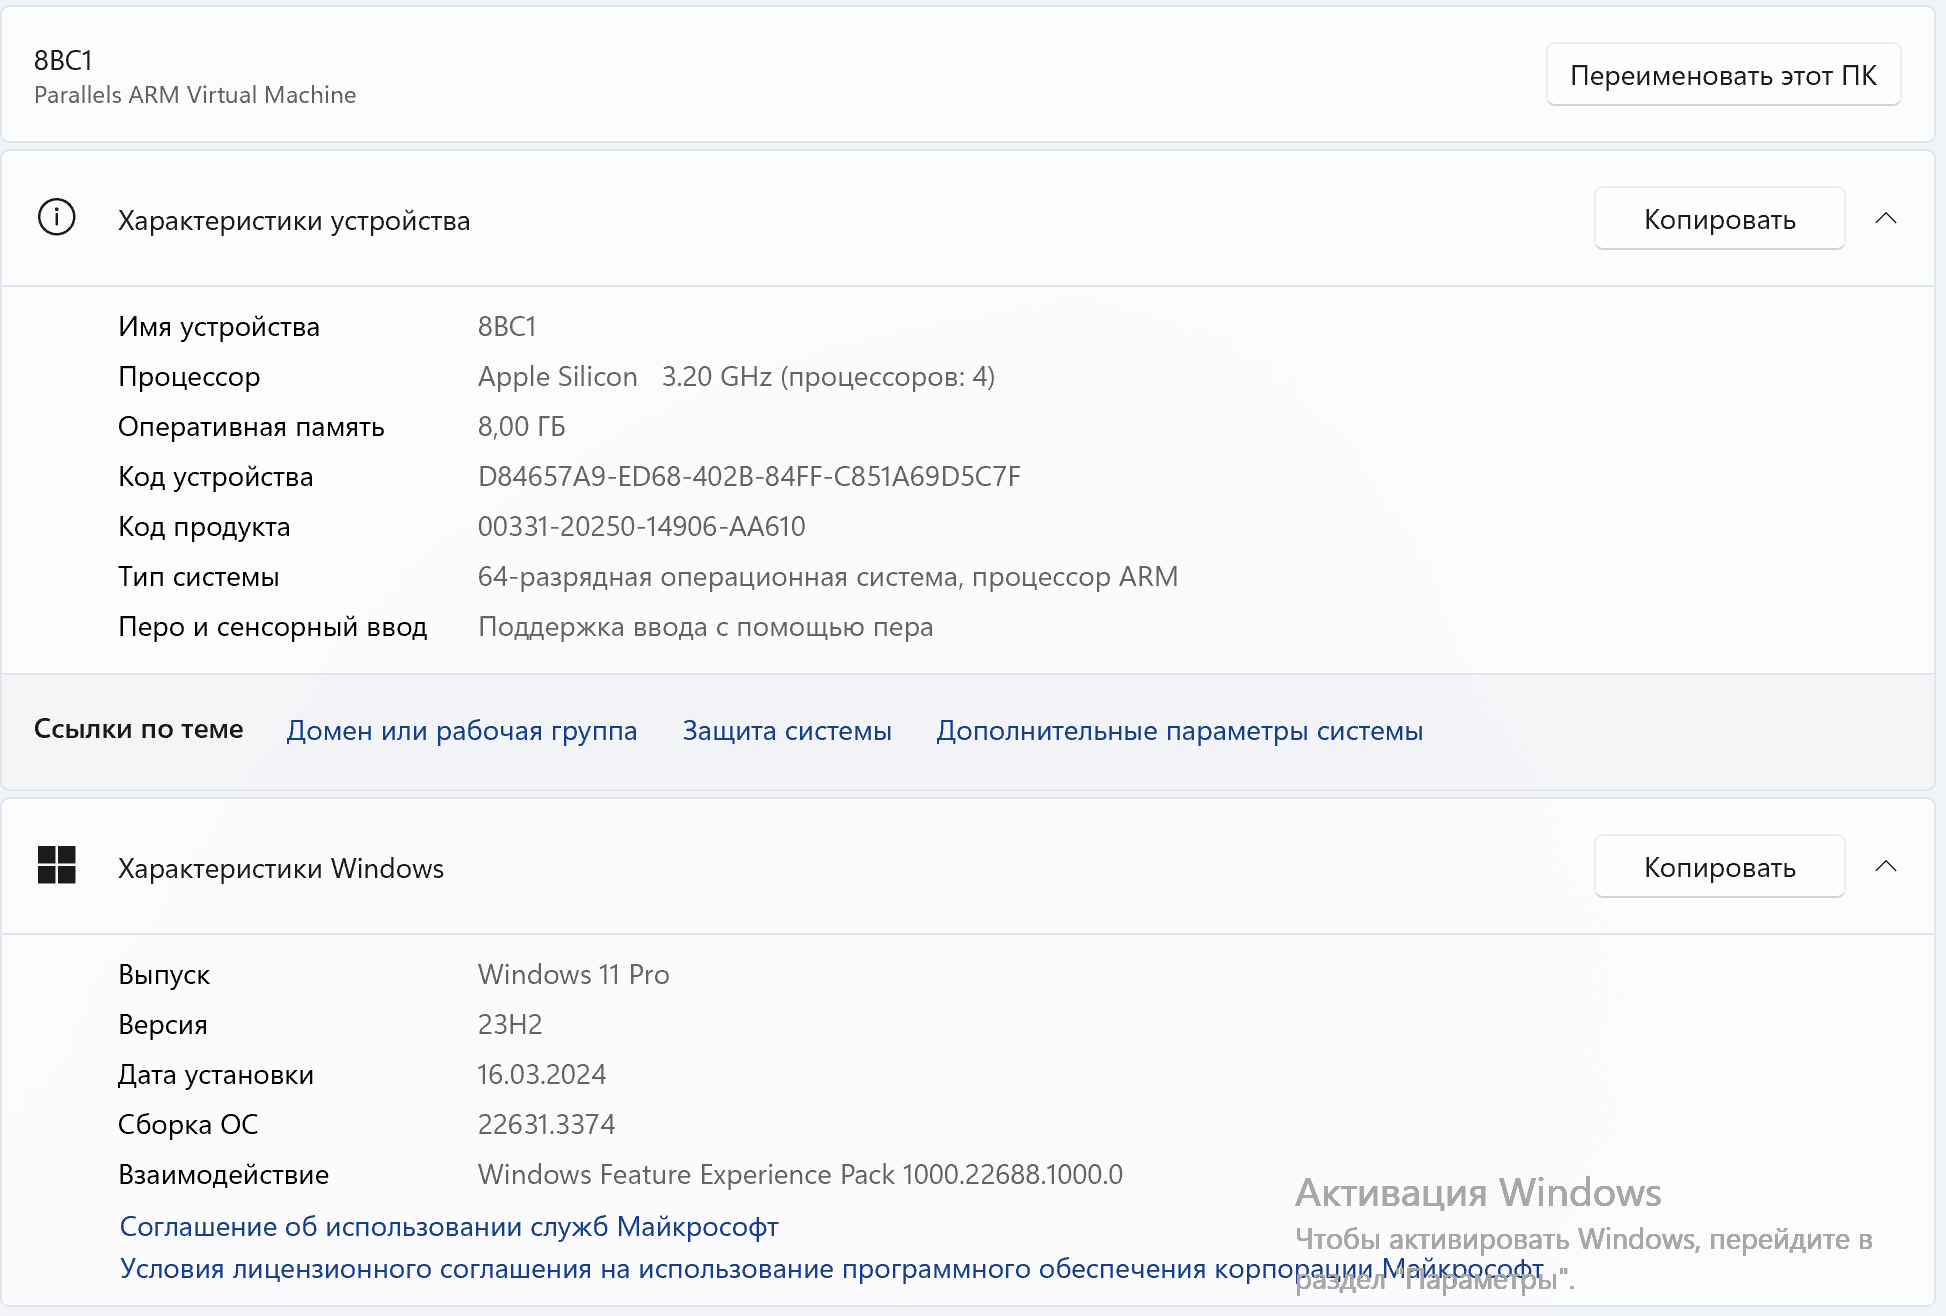
\includegraphics[width=0.8\textwidth]{../images/vm_specs.png}
    \caption{Характеристики системы}
\end{figure}
\nchapter{Основная часть}
Открыть реестр можно несколькими способами.


\textbf{Способ 1: Использование поиска в Windows}
\begin{itemize}
    \item Нажмите на кнопку «Пуск» (или нажмите клавишу Win на клавиатуре).
    \item В строке поиска введите «реестр» или «редактор реестра».
    \item В результатах поиска появится приложение «Редактор реестра» (Regedit).
    \item Нажмите на него, чтобы открыть.
\end{itemize}

\textbf{Способ 2: Использование команды «Выполнить»}
\begin{itemize}
    \item Нажмите сочетание клавиш Win + R, чтобы открыть окно «Выполнить».
    \item {Введите команду: \verb|regedit|}
    \item Нажмите Enter или кнопку «ОК».
\end{itemize}
\begin{figure}[H]
    \centering
    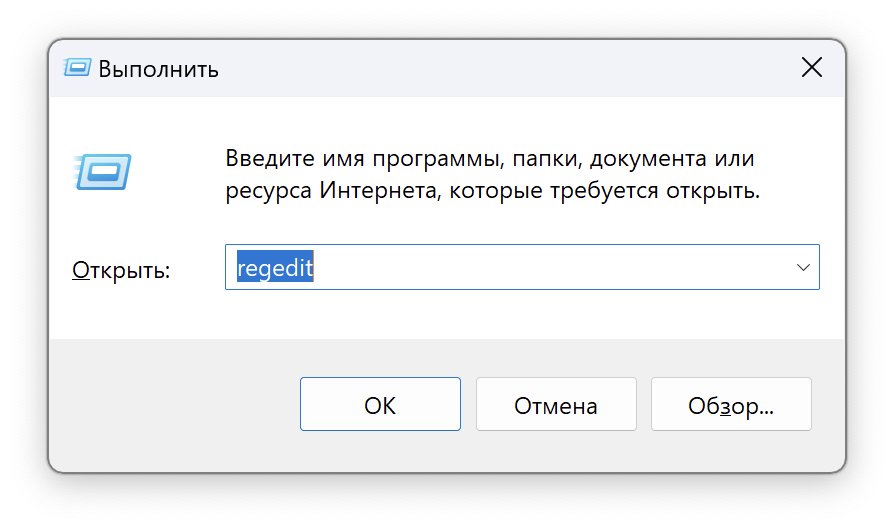
\includegraphics[width=0.8\textwidth]{../images/exec-regedit.png}
    \caption{Выполнение команды}
\end{figure}


\textbf{Способ 3: Использование PowerShell или CMD}
\begin{itemize}
    \item Откройте PowerShell или командную строку (CMD)
    \item {Введите команду: \verb|regedit|}
    \item Нажмите Enter.
\end{itemize}
\begin{figure}[H]
    \centering
    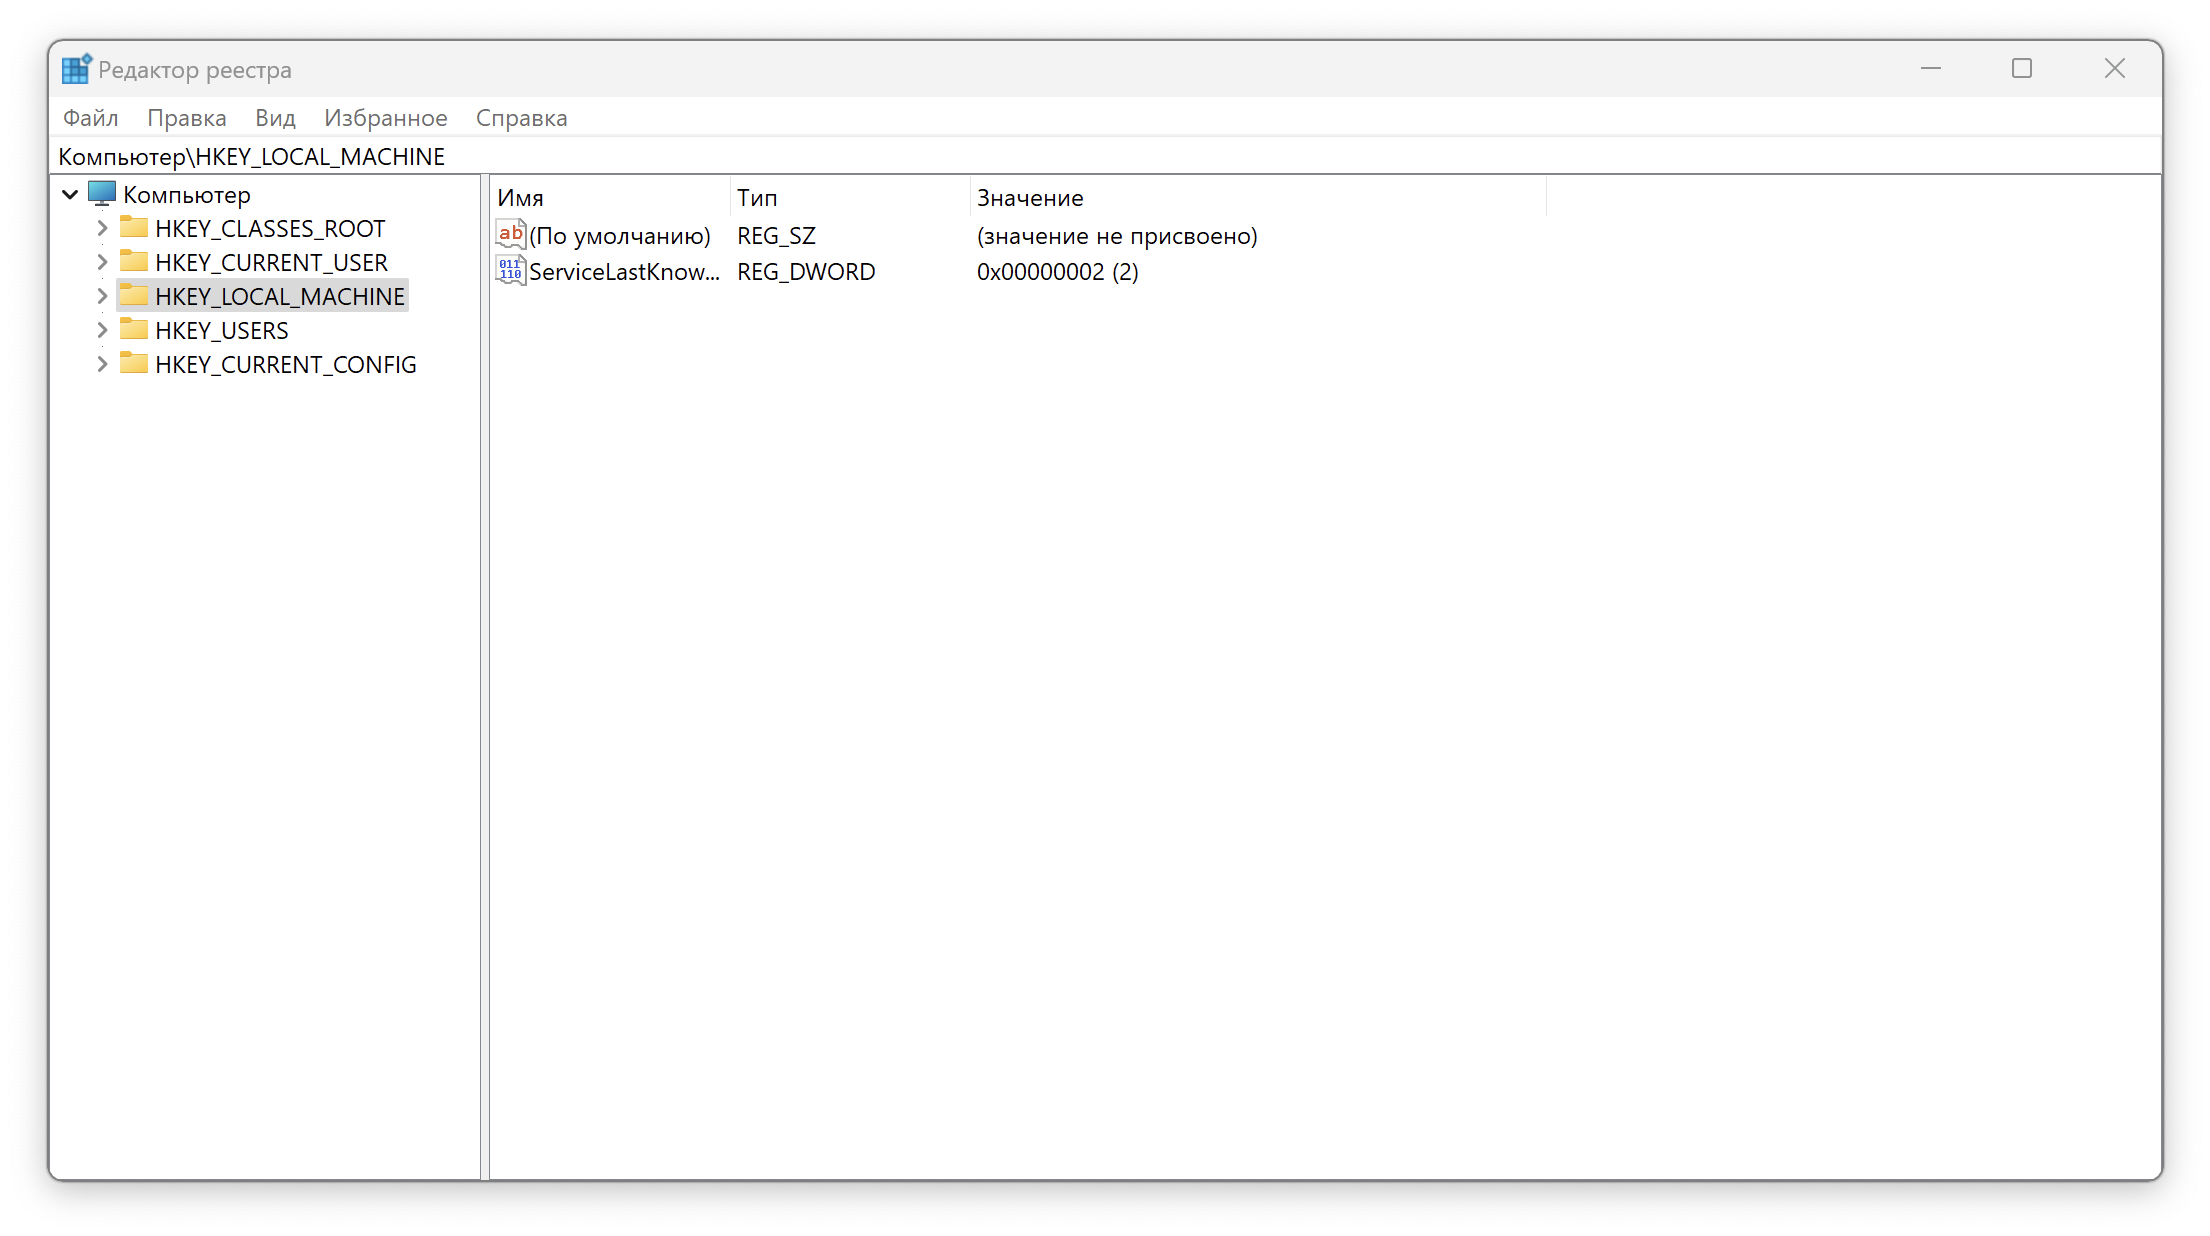
\includegraphics[width=0.8\textwidth]{../images/regedit.png}
    \caption{Системный реестр}
\end{figure}
В операционной системе Windows 10 доступ к разделам и ключам системного реестра регулируется с помощью списков контроля доступа (ACL),
определяющих права различных учетных записей и групп.
Основные учетные записи, участвующие в управлении реестром, включают:
\begin{itemize}
    \item \textbf{SYSTEM}: системная учетная запись, обладающая максимальными привилегиями.
    \item \textbf{Администраторы}: группа пользователей с правами администратора.
    \item \textbf{Пользователи}: стандартные учетные записи без административных привилегий.
\end{itemize}

\section{Рассмотрим основные ветви реестра и типичный уровень доступа к ним:}
\begin{enumerate}
    \item {\textbf{HKEY\_CURRENT\_USER}: Это ссылка на определённый подраздел HKEY\_USERS. Хранит настройки текущего пользователя.
          \begin{tcolorbox}[colback=white!95!gray, colframe=black, title=Права доступа]
              \textbf{SYSTEM}: полный доступ.\\
              \textbf{Администраторы}: полный доступ.\\
              \textbf{Пользователи}: полный доступ.
          \end{tcolorbox}

          \begin{itemize}
              \item Содержит настройки, специфичные для текущего пользователя.
              \item {Разберем некоторые из «кустов»:
                    \begin{itemize}
                        \item {\textbf{Software} — настройки программ, установленных для текущего пользователя.
                              \begin{figure}[H]
                                  \centering
                                  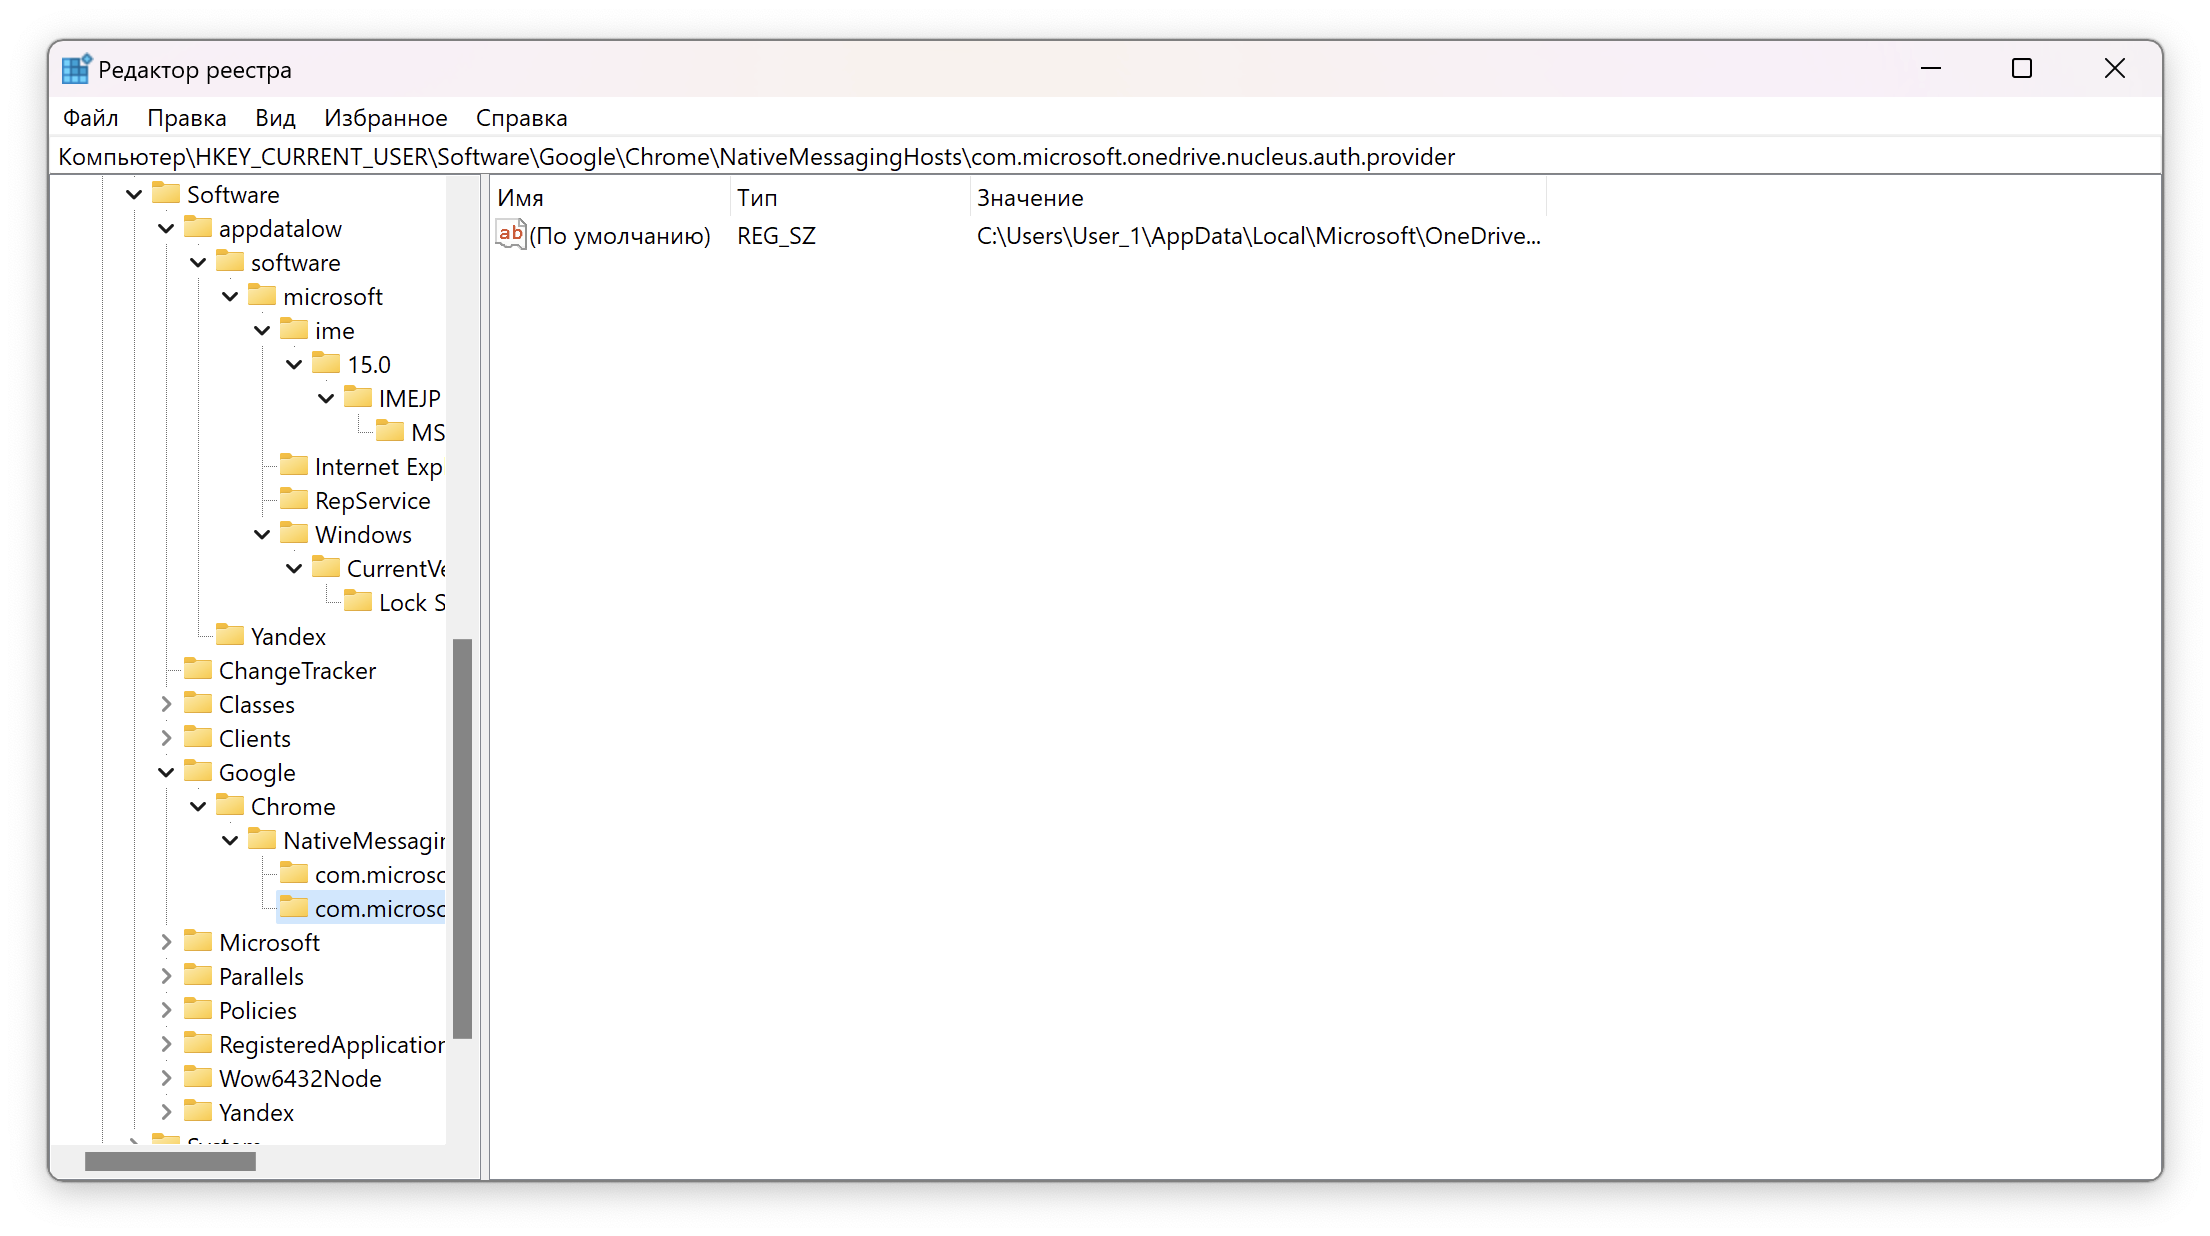
\includegraphics[width=0.8\textwidth]{../images/HKCU_software.png}
                                  \caption{Настройки программ}
                              \end{figure}
                              }
                        \item {\textbf{Control Panel} — параметры системы.
                              \begin{figure}[H]
                                  \centering
                                  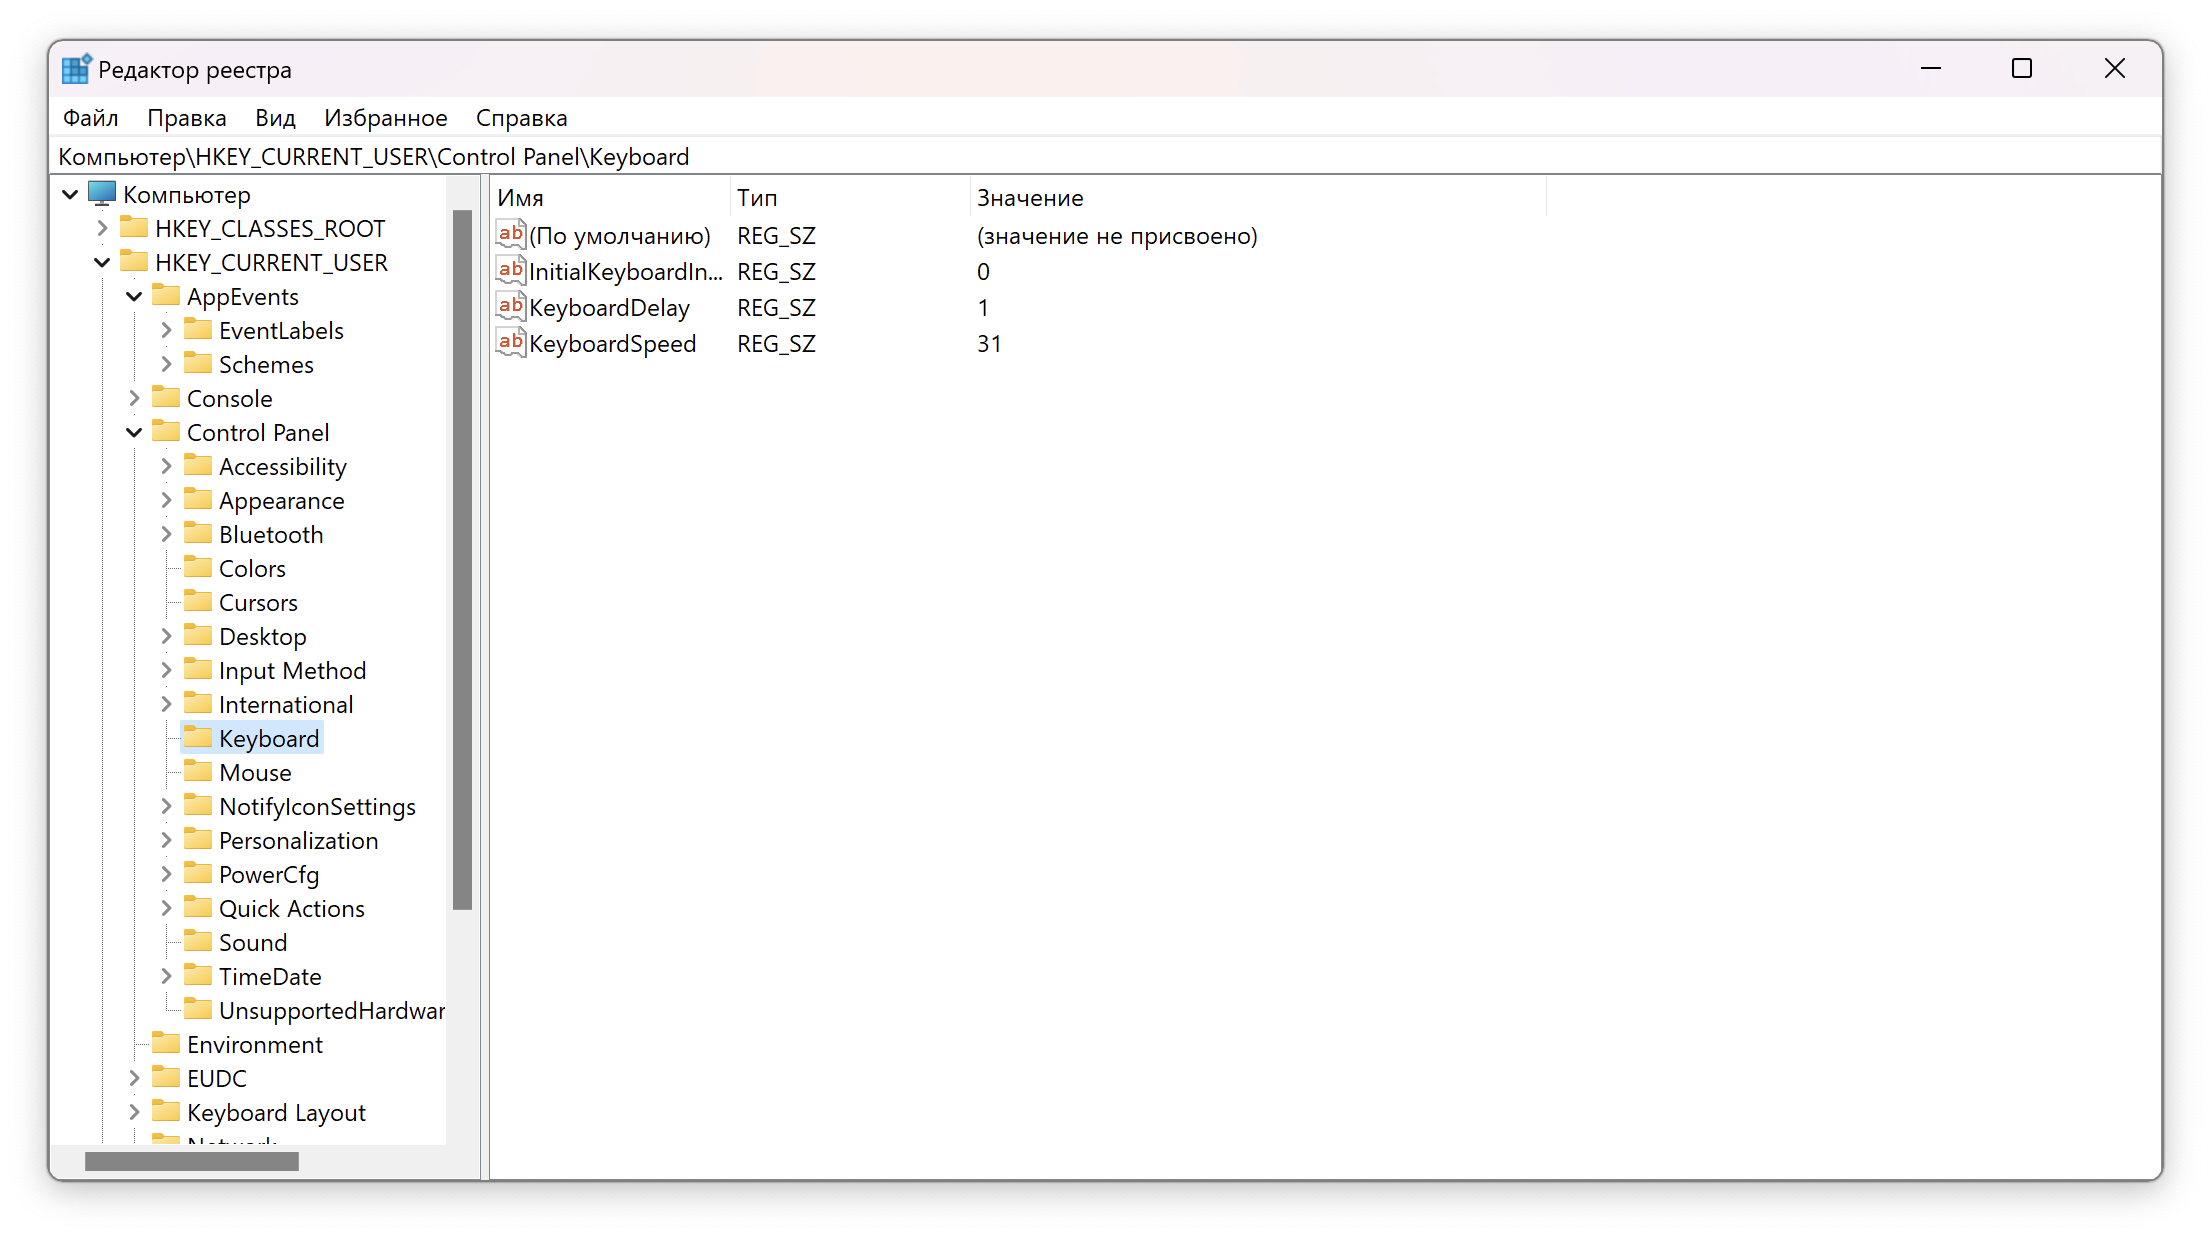
\includegraphics[width=0.8\textwidth]{../images/HKCU_control.png}
                                  \caption{Панель управления}
                              \end{figure}
                              }
                        \item {\textbf{Environment} — переменные среды, специфичные для пользователя.
                              \begin{figure}[H]
                                  \centering
                                  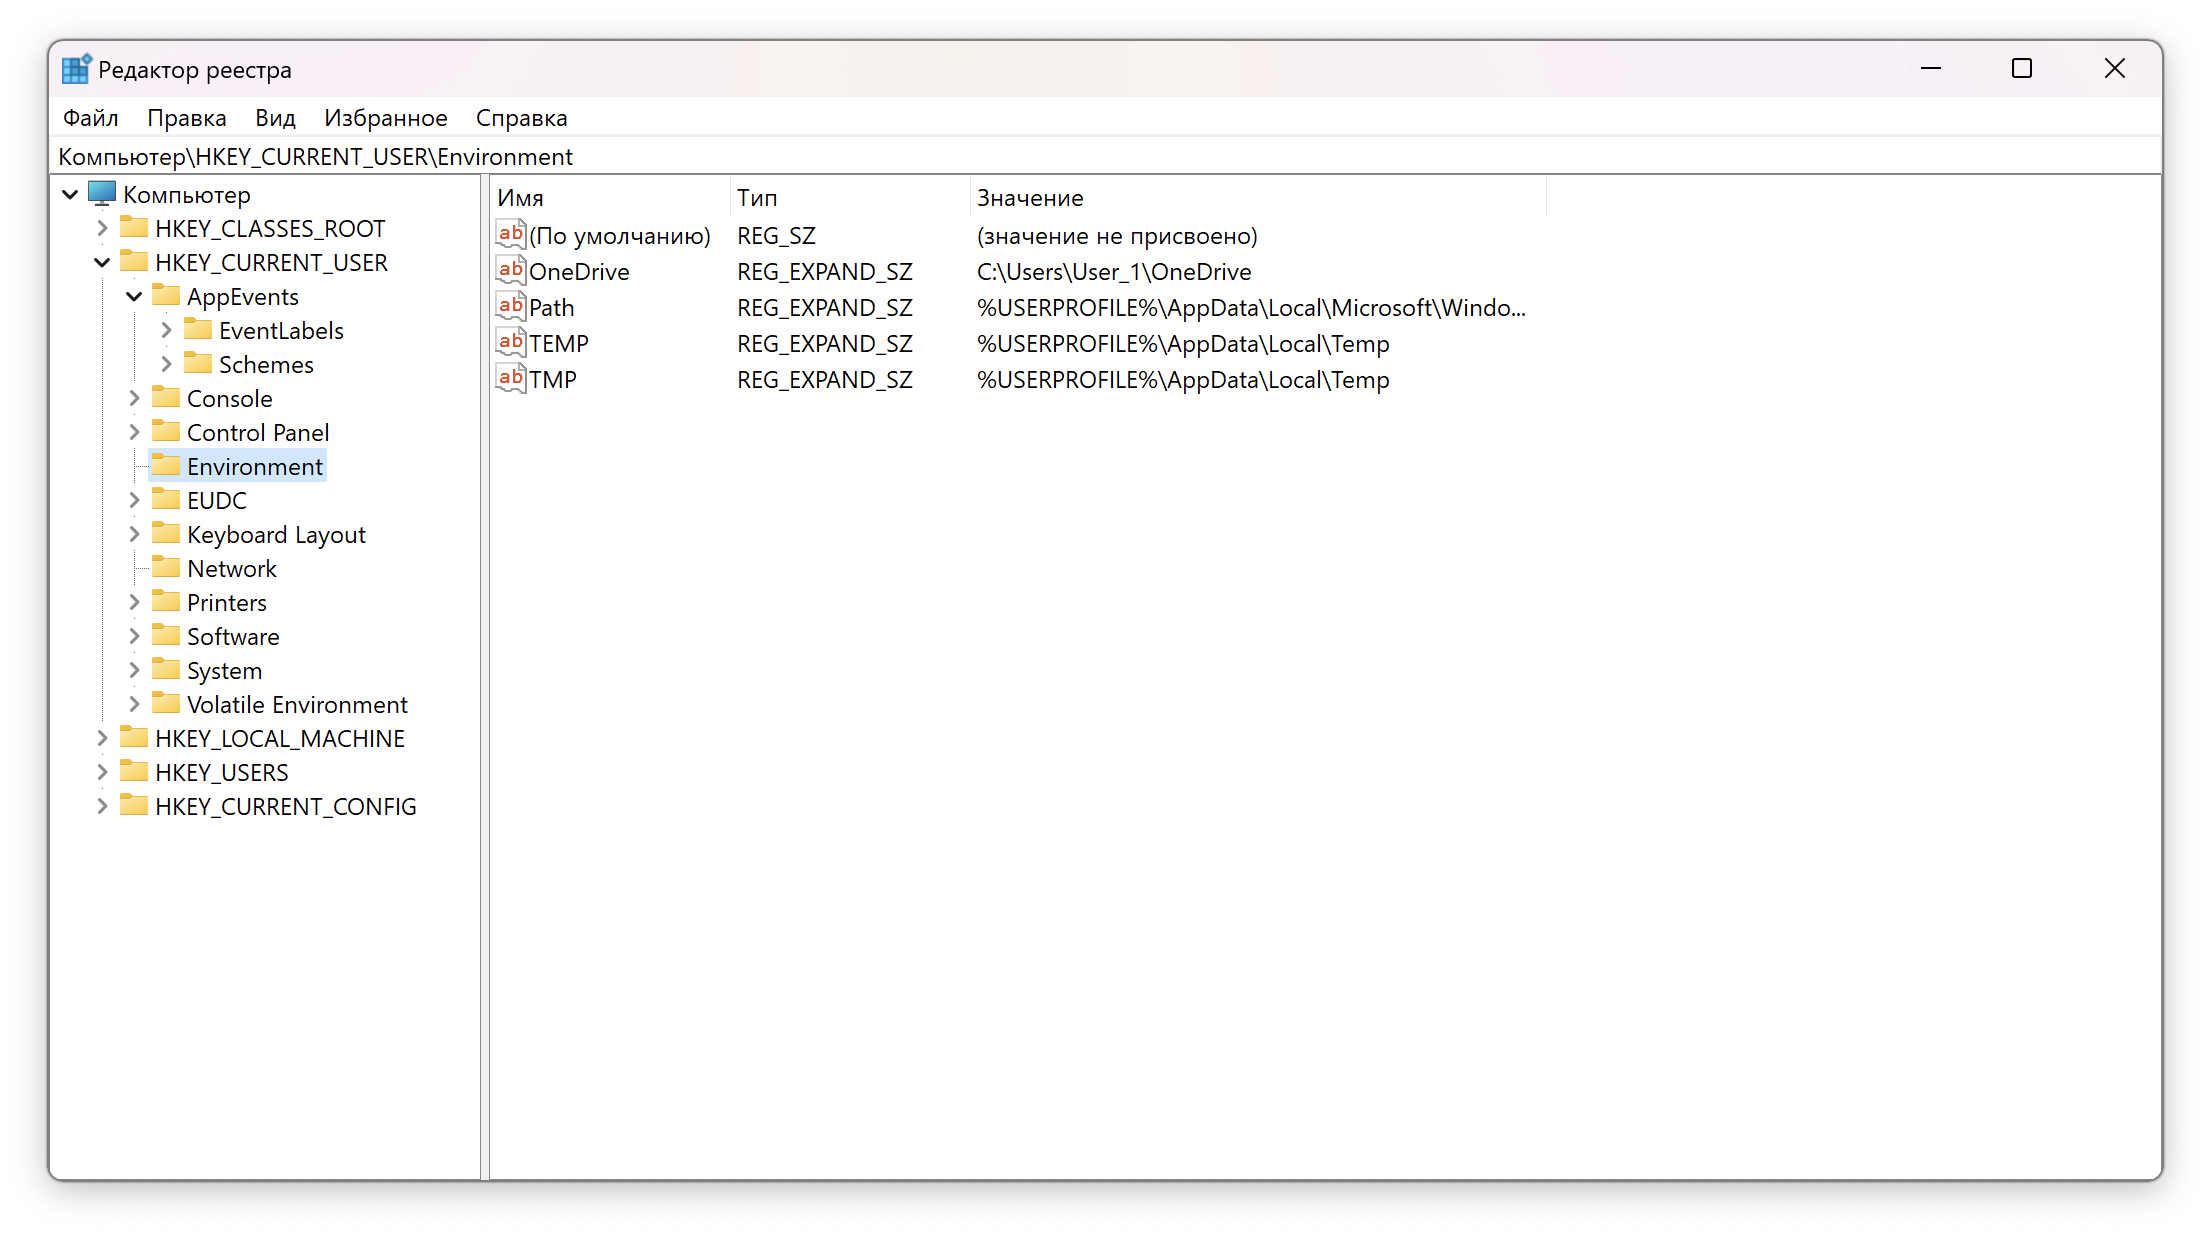
\includegraphics[width=0.8\textwidth]{../images/HKCU_env.png}
                                  \caption{Переменные среды}
                              \end{figure}
                              }


                    \end{itemize}
                    }
              \item {Вот так можно изменять значения в реестре от имени обычного пользователя:
                    \begin{figure}[H]
                        \centering
                        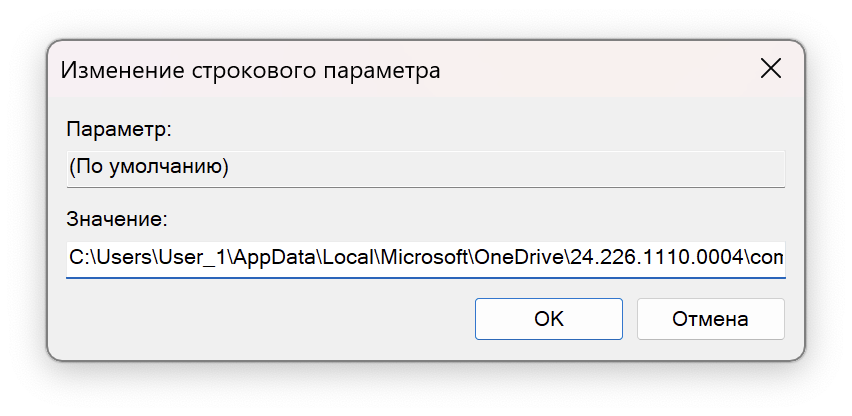
\includegraphics[width=0.8\textwidth]{../images/HKCU_regedit.png}
                        \caption{Изменение значения}
                    \end{figure}
                    }
          \end{itemize}
          }
    \item {\textbf{HKEY\_LOCAL\_MACHINE}: Раздел содержит настройки, относящиеся к вашему компьютеру и действительны для всех пользователей. Раздел содержит информацию об аппаратной конфигурации и установленном программном обеспечении.
          \begin{tcolorbox}[colback=white!95!gray, colframe=black, title=Права доступа]
              \textbf{SYSTEM}: полный доступ.\\
              \textbf{Администраторы}: частичный доступ.\\
              \textbf{Пользователи}: большинство доступно для чтения, есть недоступные разделы, есть разделы с полным доступом.
          \end{tcolorbox}
          \begin{itemize}
              \item {Разберем некоторые из «кустов»:
                    \begin{itemize}
                        \item \textbf{Software} — глобальные настройки программ.
                        \item \textbf{System} — настройки текущей конфигурации системы.
                        \item \textbf{Hardware} — описание аппаратного обеспечения (динамическая ветка, создается при запросе).
                        \item \textbf{SAM} — данные о пользователях и группах (Security Accounts Manager). Недоступна для обычных пользователей.
                        \item \textbf{Security} — политики безопасности. Недоступна для обычных пользователей.
                    \end{itemize}
                    }
              \item {Отказ в доступе пользователю:
                    \begin{figure}[H]
                        \centering
                        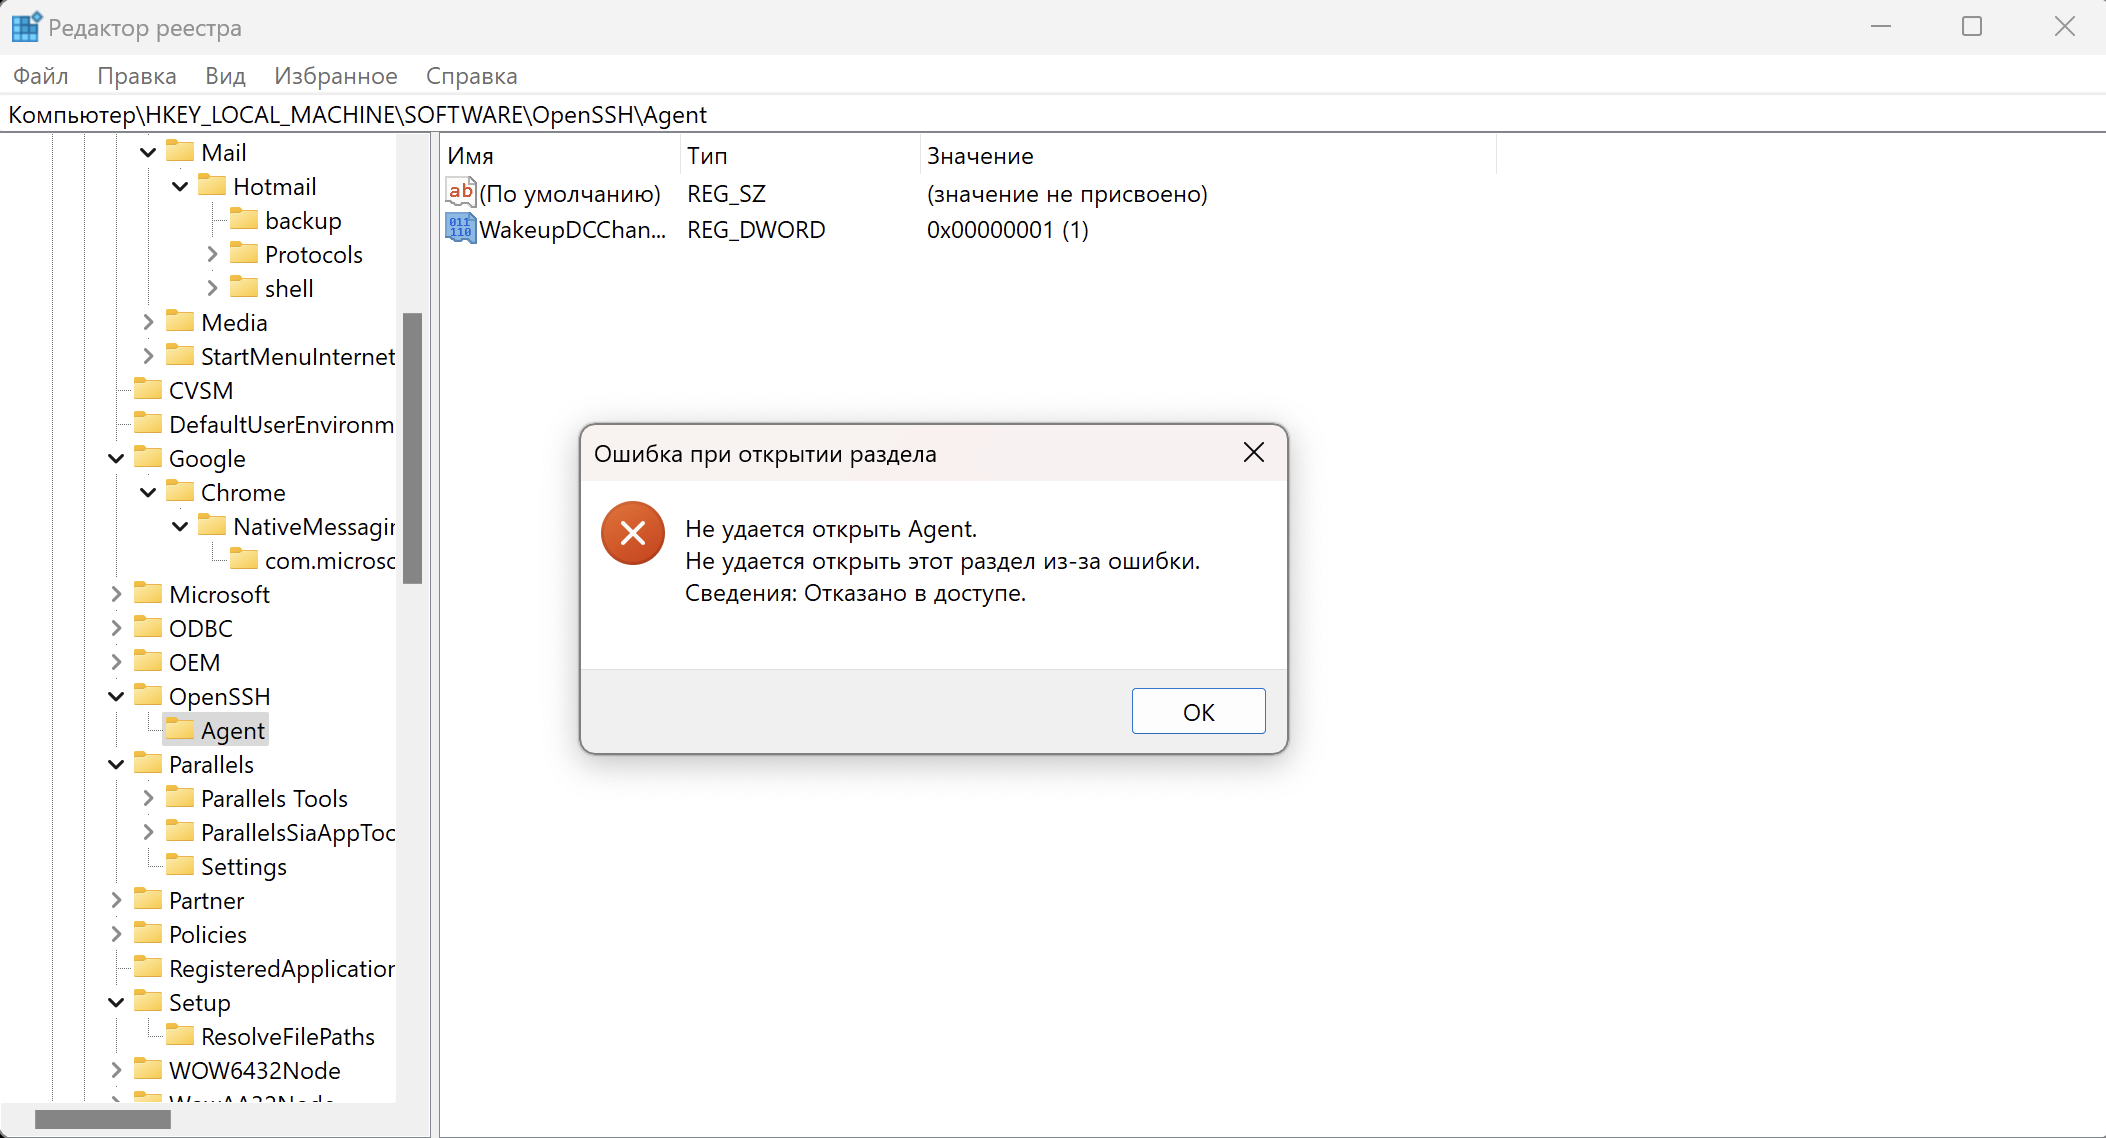
\includegraphics[width=0.8\textwidth]{../images/HKLM_denied.png}
                        \caption{Отказ в доступе в OpenSSH/Agent}
                    \end{figure}
                    }
              \item {Отказ на редактирование администратору:
                    \begin{figure}[H]
                        \centering
                        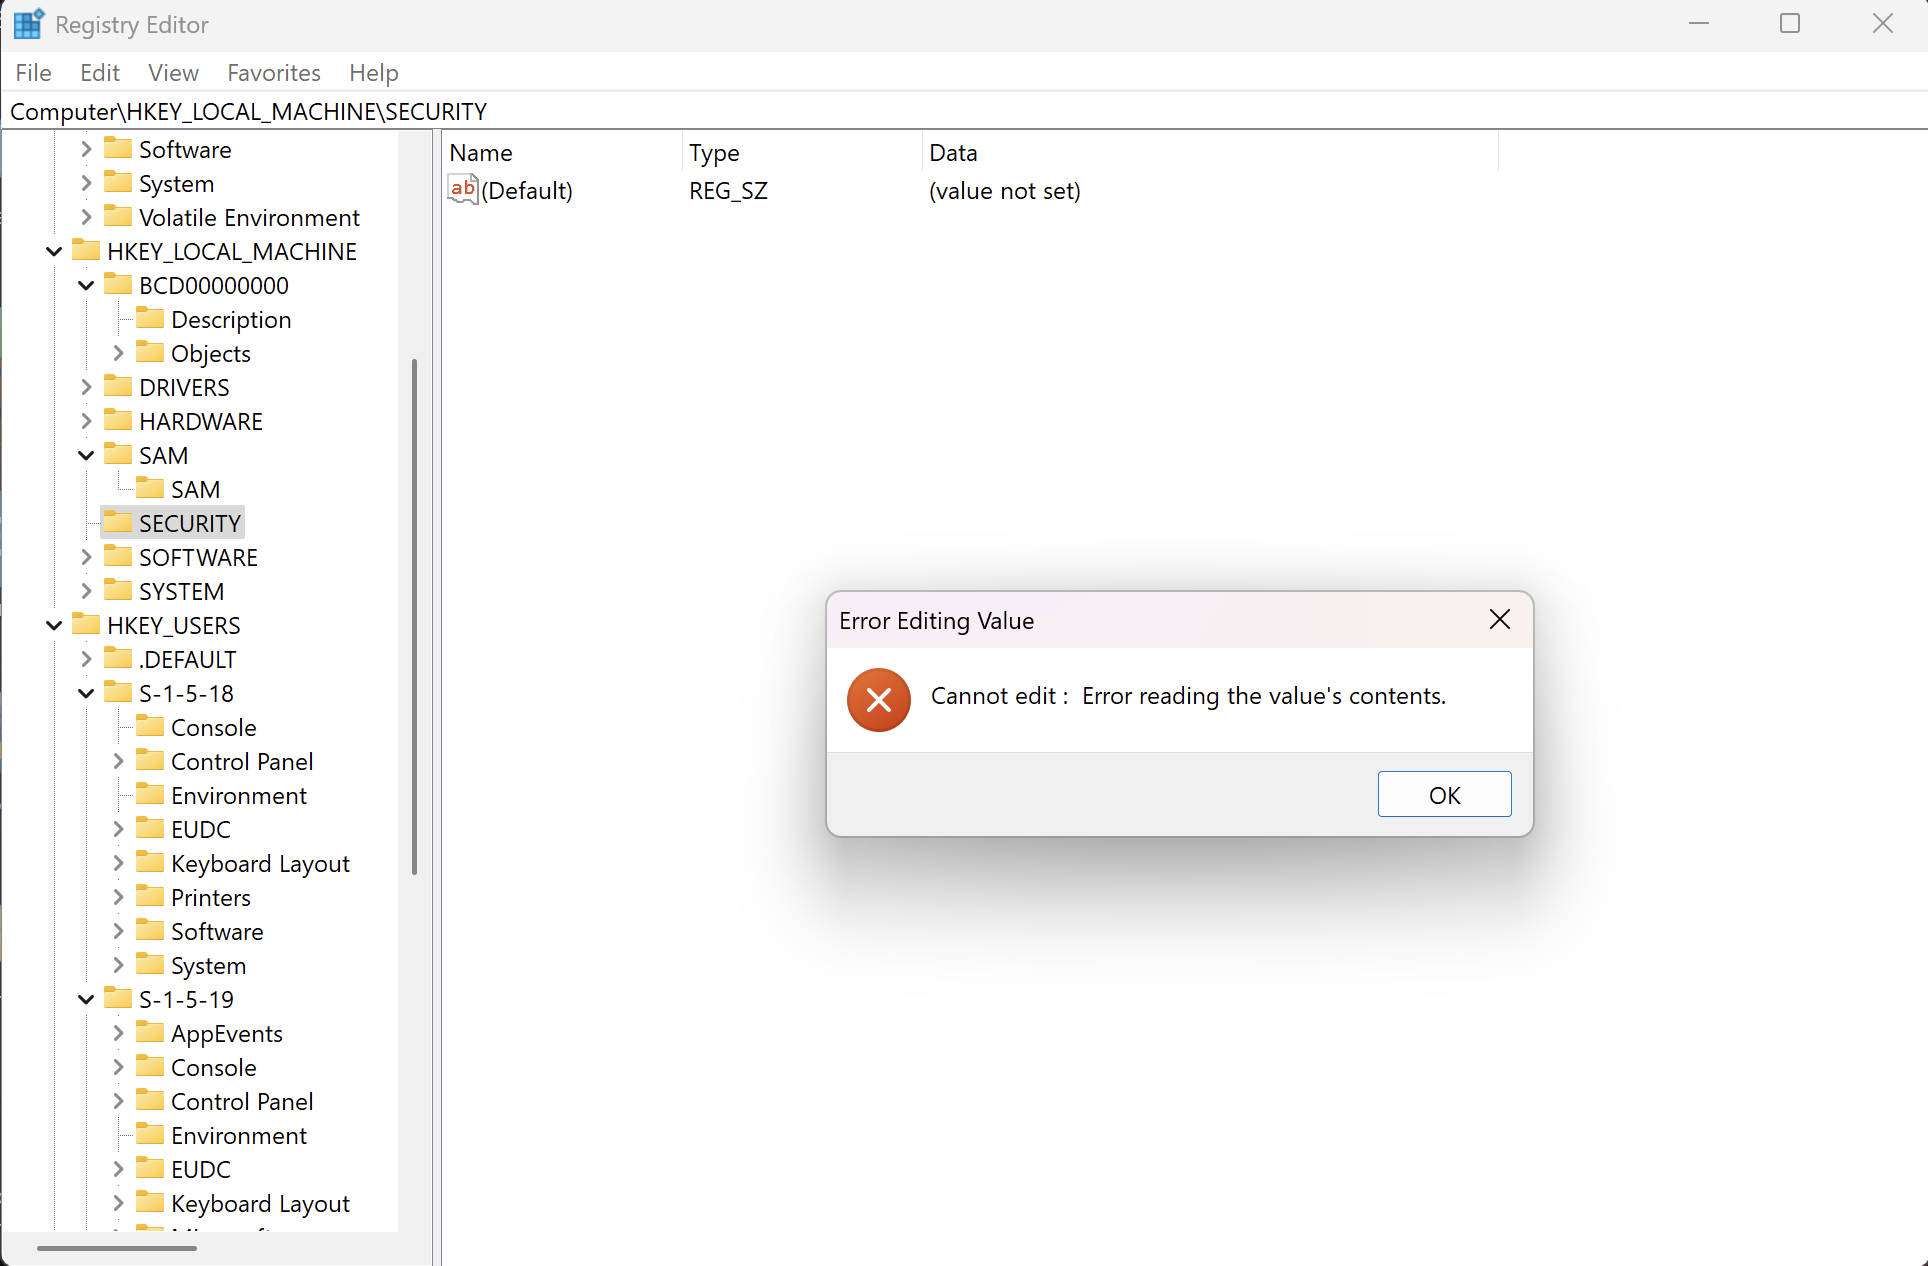
\includegraphics[width=0.8\textwidth]{../images/HKLM_admin.png}
                        \caption{Отказ на редактирование Security}
                    \end{figure}}
          \end{itemize}
          }
    \item {\textbf{HKEY\_USERS}: Этот раздел содержит настройки для всех пользователей компьютера
          \begin{tcolorbox}[colback=white!95!gray, colframe=black, title=Права доступа]
              \textbf{SYSTEM}: полный доступ.\\
              \textbf{Администраторы}: полный доступ.\\
              \textbf{Пользователи}: Пользователь может просматривать только данные соответсвующие его SID.
          \end{tcolorbox}
          }
    \item {\textbf{HKEY\_CURRENT\_CONFIG}: Это ссылка на HKEY\_LOCAL\_MACHINE$\backslash$SYSTEM$\backslash$Current ControlSet$\backslash$Hardware Profiles$\backslash$Current. Раздел содержит сведения о настройках оборудования, используемом локальным компьютером при запуске системы, т.е. содержит информацию о текущей конфигурации.
          \begin{tcolorbox}[colback=white!95!gray, colframe=black, title=Права доступа]
              \textbf{SYSTEM}: полный доступ.\\
              \textbf{Администраторы}: полный доступ.\\
              \textbf{Пользователи}: чтение.
          \end{tcolorbox}
          \begin{figure}[H]
              \centering
              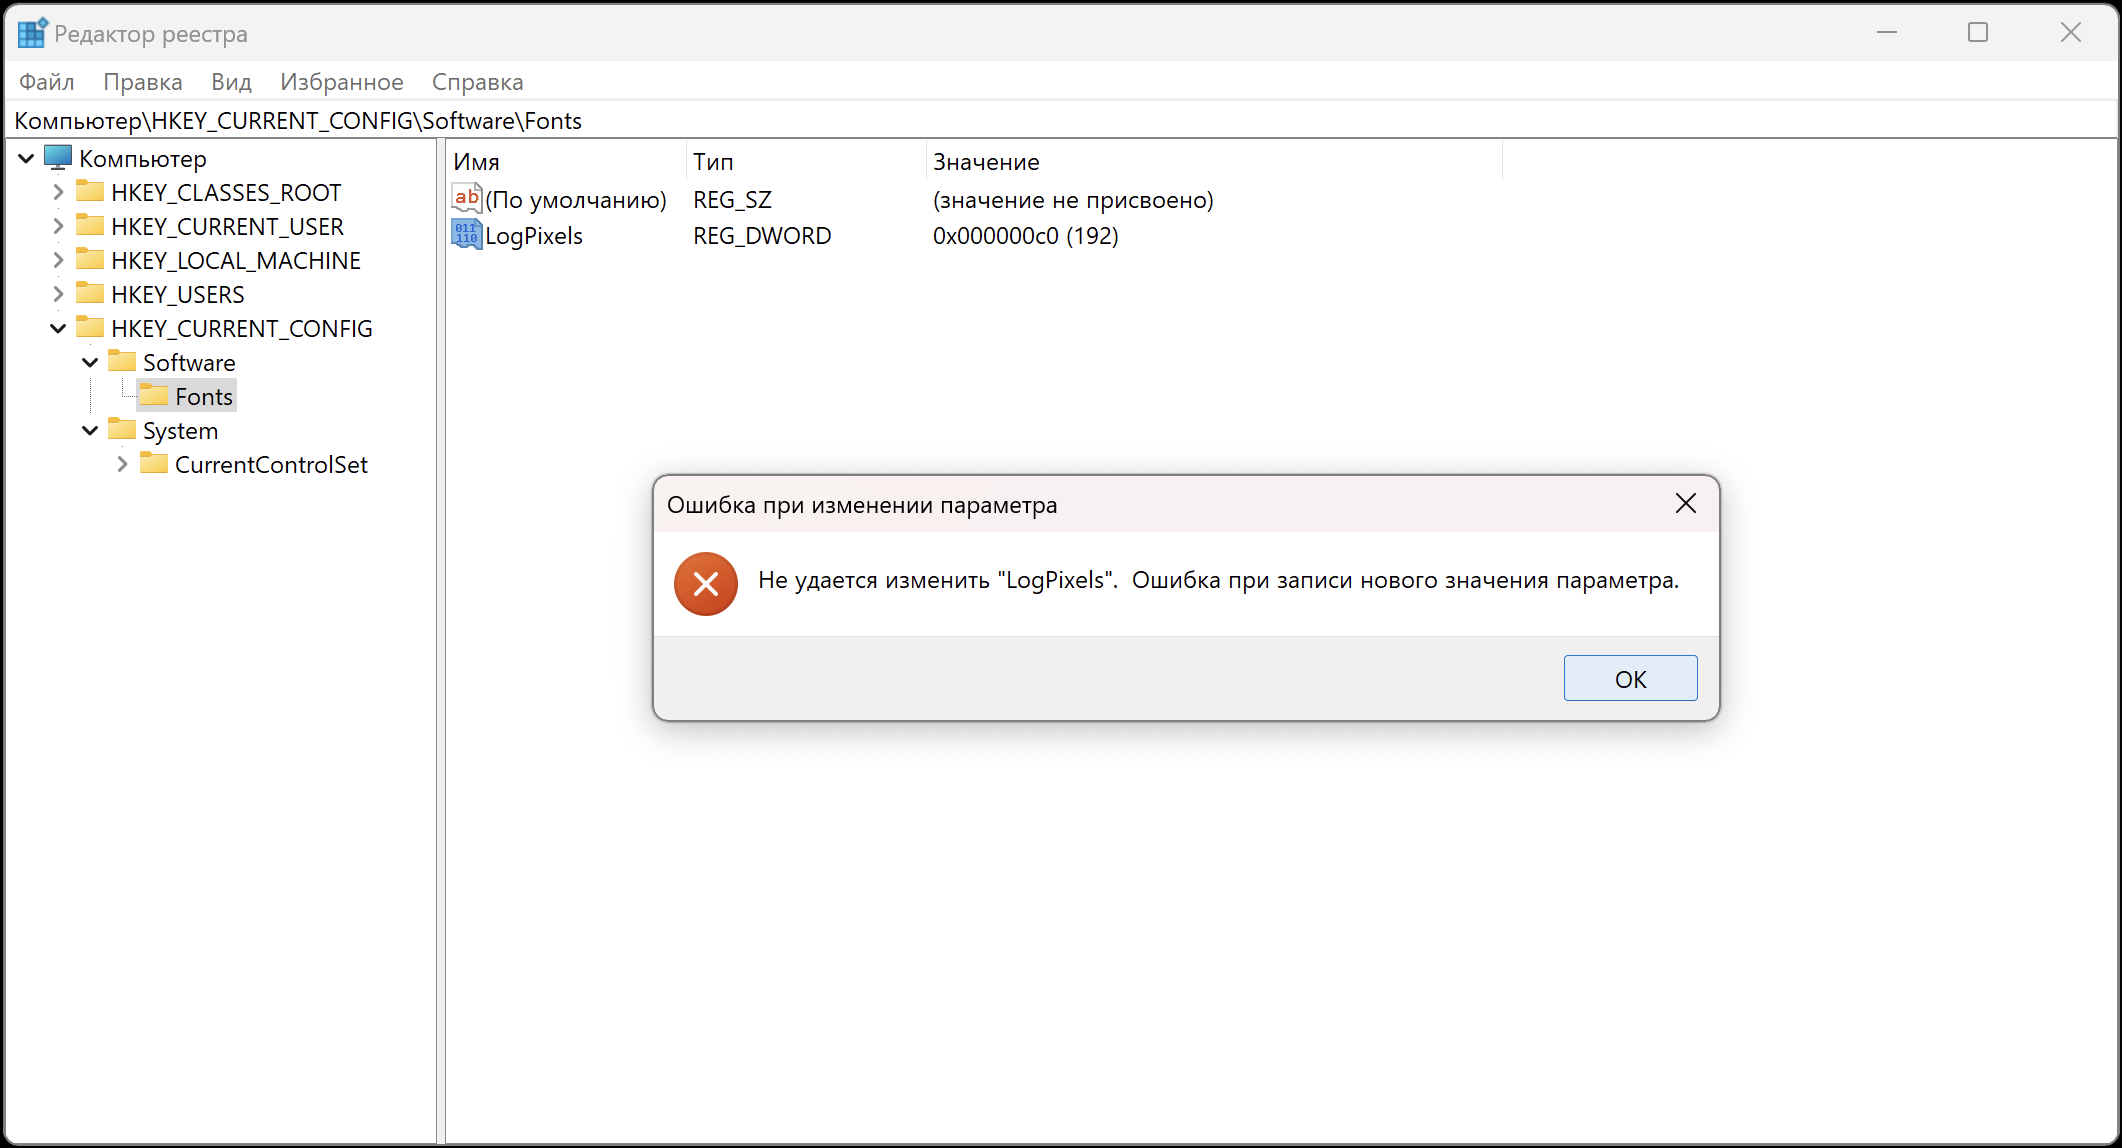
\includegraphics[width=0.8\textwidth]{../images/HKCC_users.png}
              \caption{Обычному пользователю доступно только чтение}
          \end{figure}
          }
    \item {\textbf{HKEY\_CLASSES\_ROOT}: Отображает данные из HKEY\_LOCAL\_MACHINE$\backslash$ Software$\backslash$Classes и HKEY\_CURRENT\_USER$\backslash$Software$\backslash$Classes. Хранящиеся здесь сведения обеспечивают запуск необходимой программы при открытии файла с помощью проводника. Этот раздел содержит связи между приложениями и типами файлов, а также информацию об OLE.
          \begin{tcolorbox}[colback=white!95!gray, colframe=black, title=Права доступа]
              \textbf{SYSTEM}: полный доступ.\\
              \textbf{Администраторы}: полный доступ.\\
              \textbf{Пользователи}: чтение.
          \end{tcolorbox}
          \begin{figure}[H]
              \centering
              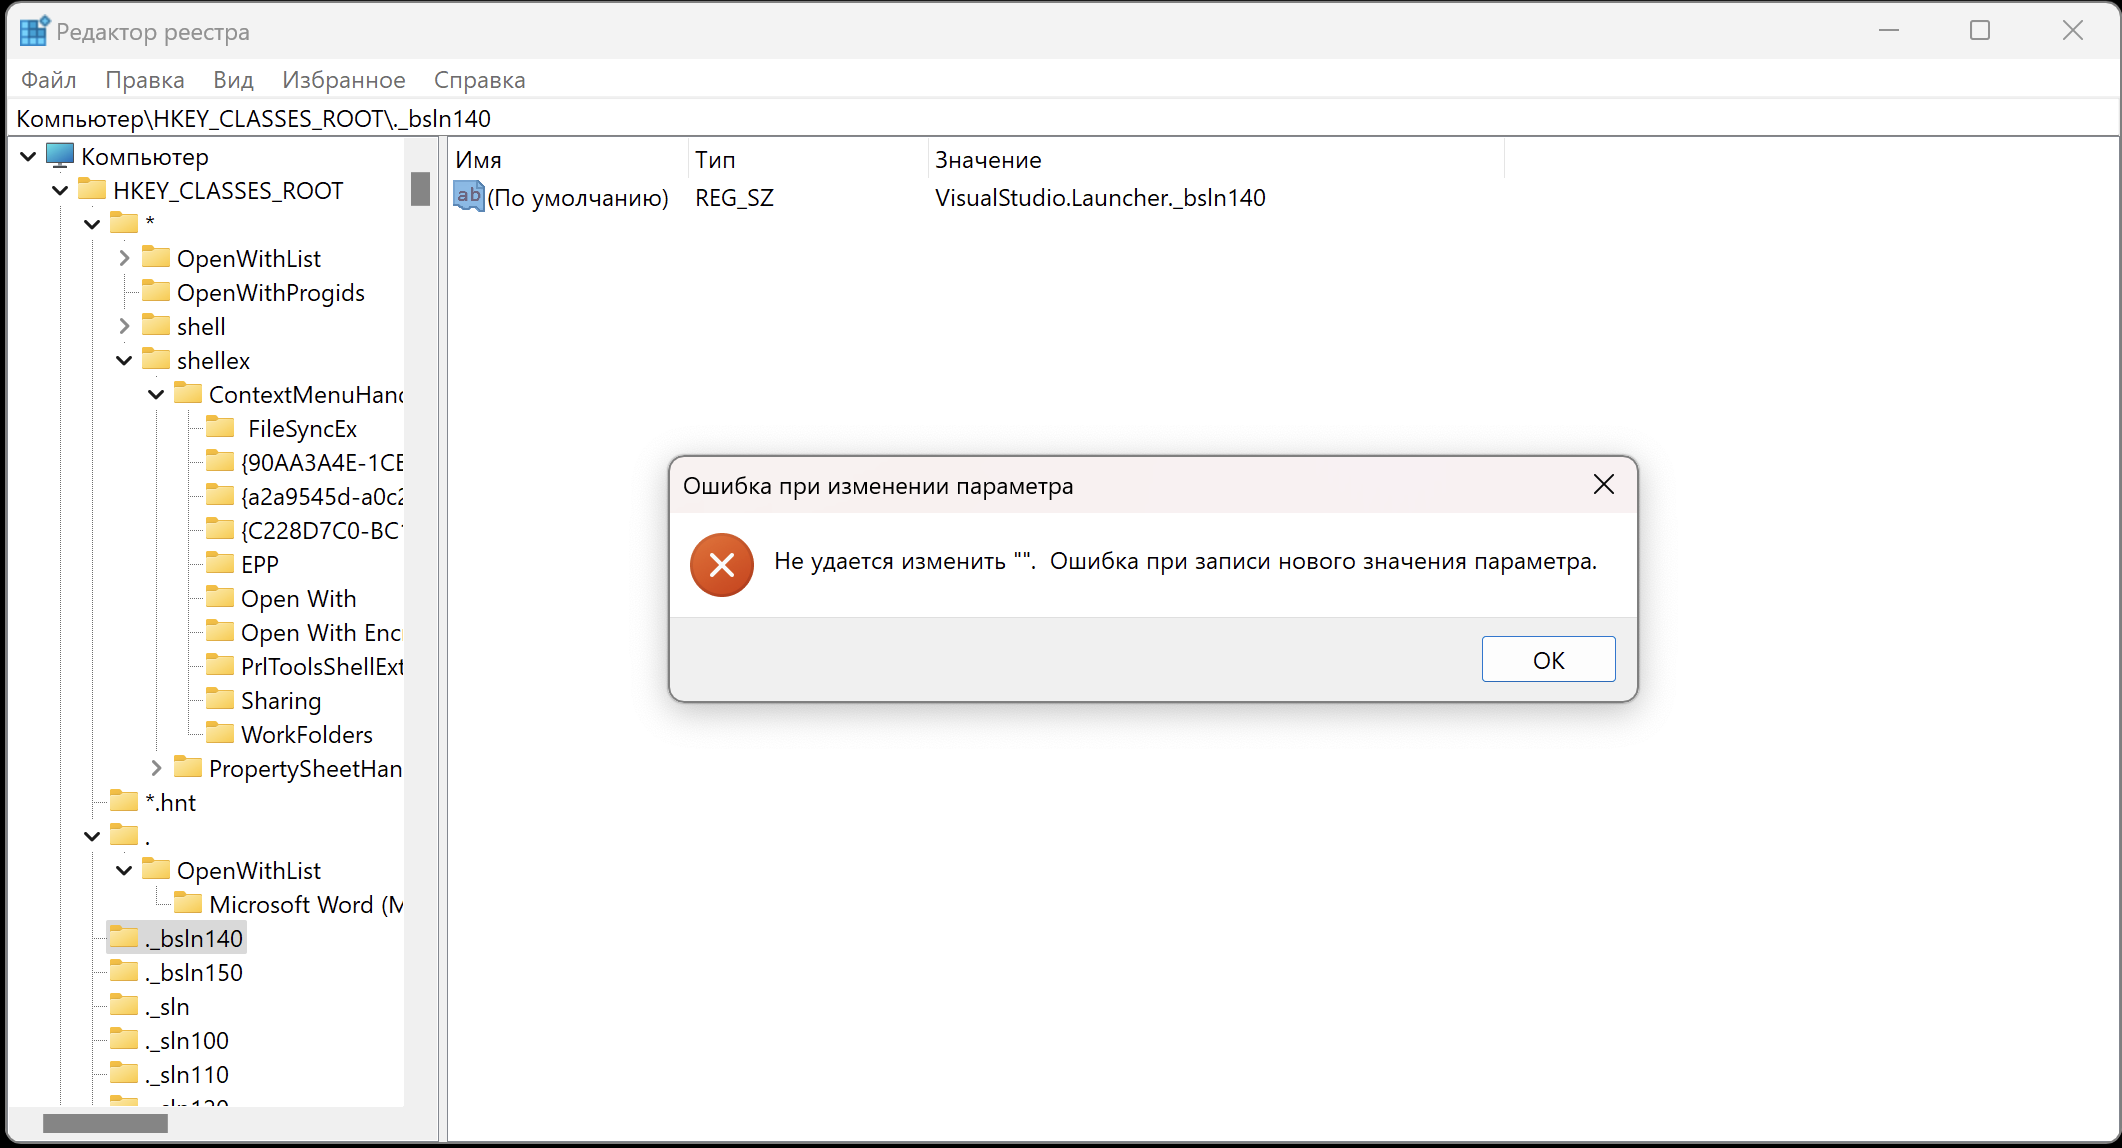
\includegraphics[width=0.8\textwidth]{../images/HKCR_users.png}
              \caption{Обычному пользователю доступно только чтение}
          \end{figure}
          }
\end{enumerate}
\section{Способы восстановления реестра}
\begin{enumerate}
    \item {\textbf{Восстановление реестра из резервной копии}
          \begin{enumerate}
              \item {Автоматически созданная резервная копия.
                    Windows автоматически создает резервные копии реестра в папке \verb|C:\Windows\System32\config\RegBack|. Эти файлы обновляются после каждого значительного обновления системы. Для восстановления реестра из резервной копии необходимо скопировать файлы из папки \verb|RegBack| в папку \verb|config|.

                    \textbf{Шаги}:
                    \begin{enumerate}
                        \item Откройте командную строку.
                        \item {Введите команду:
                              \begin{lstlisting}[language=bash]
xcopy c:\windows\system32\config\regback c:\windows\system32\config
                            \end{lstlisting}
                              }
                        \item Подтвердите замену файлов, введя \verb|A|.
                        \item Перезагрузите компьютер.
                    \end{enumerate}
                    \textbf{Важно:} Начиная с Windows 10 версии 1803, автоматическое создание резервных копий реестра отключено по умолчанию. В таком случае папка RegBack может быть пуста или содержать нулевые файлы.
                    \begin{tcolorbox}[colback=white!95!gray, colframe=black, title=Резервное копирование системного реестра в папку RegBack перестало выполняться в Windows 10 версии 1803]
                        Начиная с Windows 10, версия 1803, Windows больше не выполняет автоматическое резервное копирование системного реестра в папку RegBack. Если вы перейдете в папку \verb|\Windows\System32\config\RegBack| в проводнике Windows, вы по-прежнему увидите все ветки реестра, но каждый файл будет иметь размер 0 кб.
                        \begin{figure}[H]
                            \centering
                            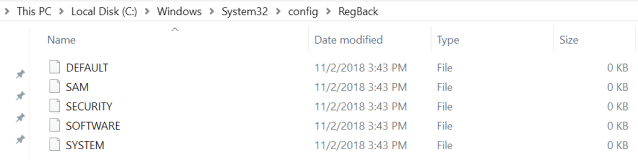
\includegraphics[width=0.8\textwidth]{../images/regisrtry-hive-0-kb.png}
                            \caption{Резервная копия реестра}
                        \end{figure}
                        Это изменение сделано специально и призвано помочь уменьшить общий размер дискового пространства Windows. Для восстановления системы с поврежденной веткой реестра Microsoft рекомендует использовать точку восстановления системы.


                        Если вам приходится использовать устаревшее поведение резервного копирования, вы можете включить его, настроив следующую запись реестра и перезагрузив компьютер:
                        \begin{itemize}
                            \item Path: \verb|HKLM\System\|
                                  \verb|CurrentControlSet\|
                                  \verb|Control\Session Manager\|
                                  \verb|Configuration Manager\|
                                  \verb|EnablePeriodicBackup|
                            \item Type: \verb|REG_DWORD|
                            \item Value: \verb|1|
                        \end{itemize}

                        Windows создает резервную копию реестра в папку \verb|RegBack| при перезагрузке компьютера и задачу \verb|RegIdleBackup| для управления последующими резервными копиями. Windows хранит информацию о задаче в библиотеке запланированных задач в папке \verb|Microsoft\|\verb|Windows\|\verb|Registry|. Задача имеет следующие свойства:
                        \begin{figure}[H]
                            \centering
                            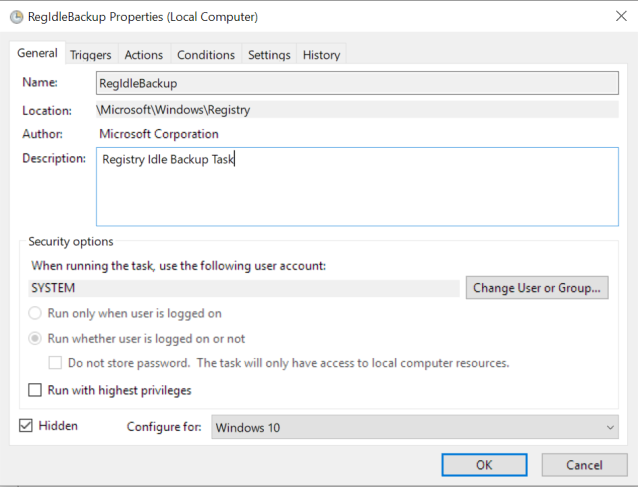
\includegraphics[width=0.8\textwidth]{../images/properties-of-regidlebackup-task.png}
                            \caption{Задача RegIdleBackup}
                        \end{figure}
                    \end{tcolorbox}
                    }
              \item {Создание собственной резервной копии.

                    Пользователь может создать резервную копию реестра вручную, чтобы использовать её в будущем.

                    \textbf{Шаги}:
                    \begin{enumerate}
                        \item Откройте редактор реестра (\verb|regedit|).
                        \item Выберите корневой раздел \verb|Компьютер|.
                        \item {Выберите в меню \verb|Файл| пункт \verb|Экспорт|.
                              \begin{figure}[H]
                                  \centering
                                  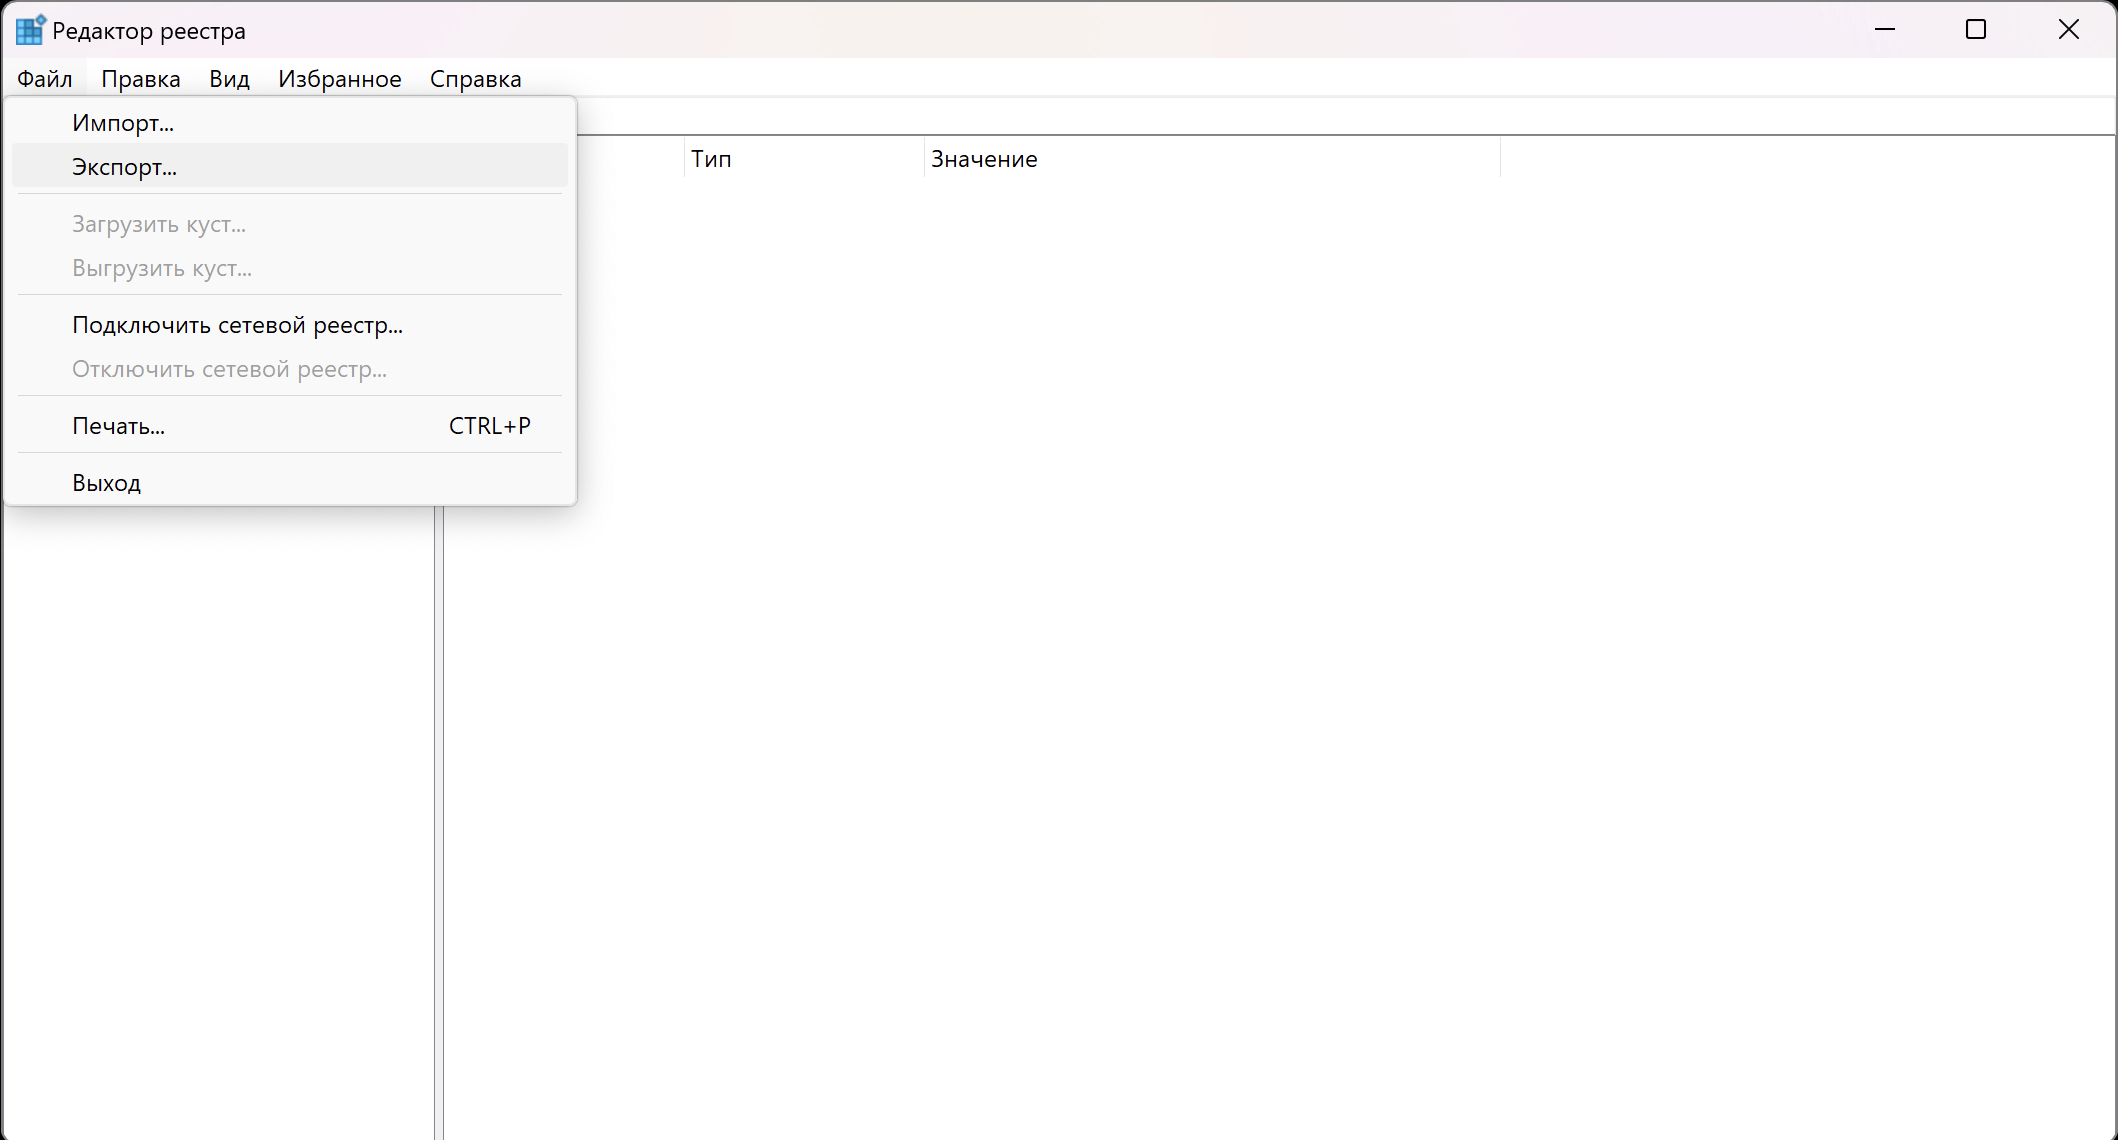
\includegraphics[width=0.8\textwidth]{../images/regedit_export.png}
                                  \caption{Экспорт реестра}
                              \end{figure}
                              }
                        \item {Для восстановления достаточно дважды кликнуть по файлу \verb|.reg| и подтвердить внесение изменений.

                              \begin{figure}[H]
                                  \centering
                                  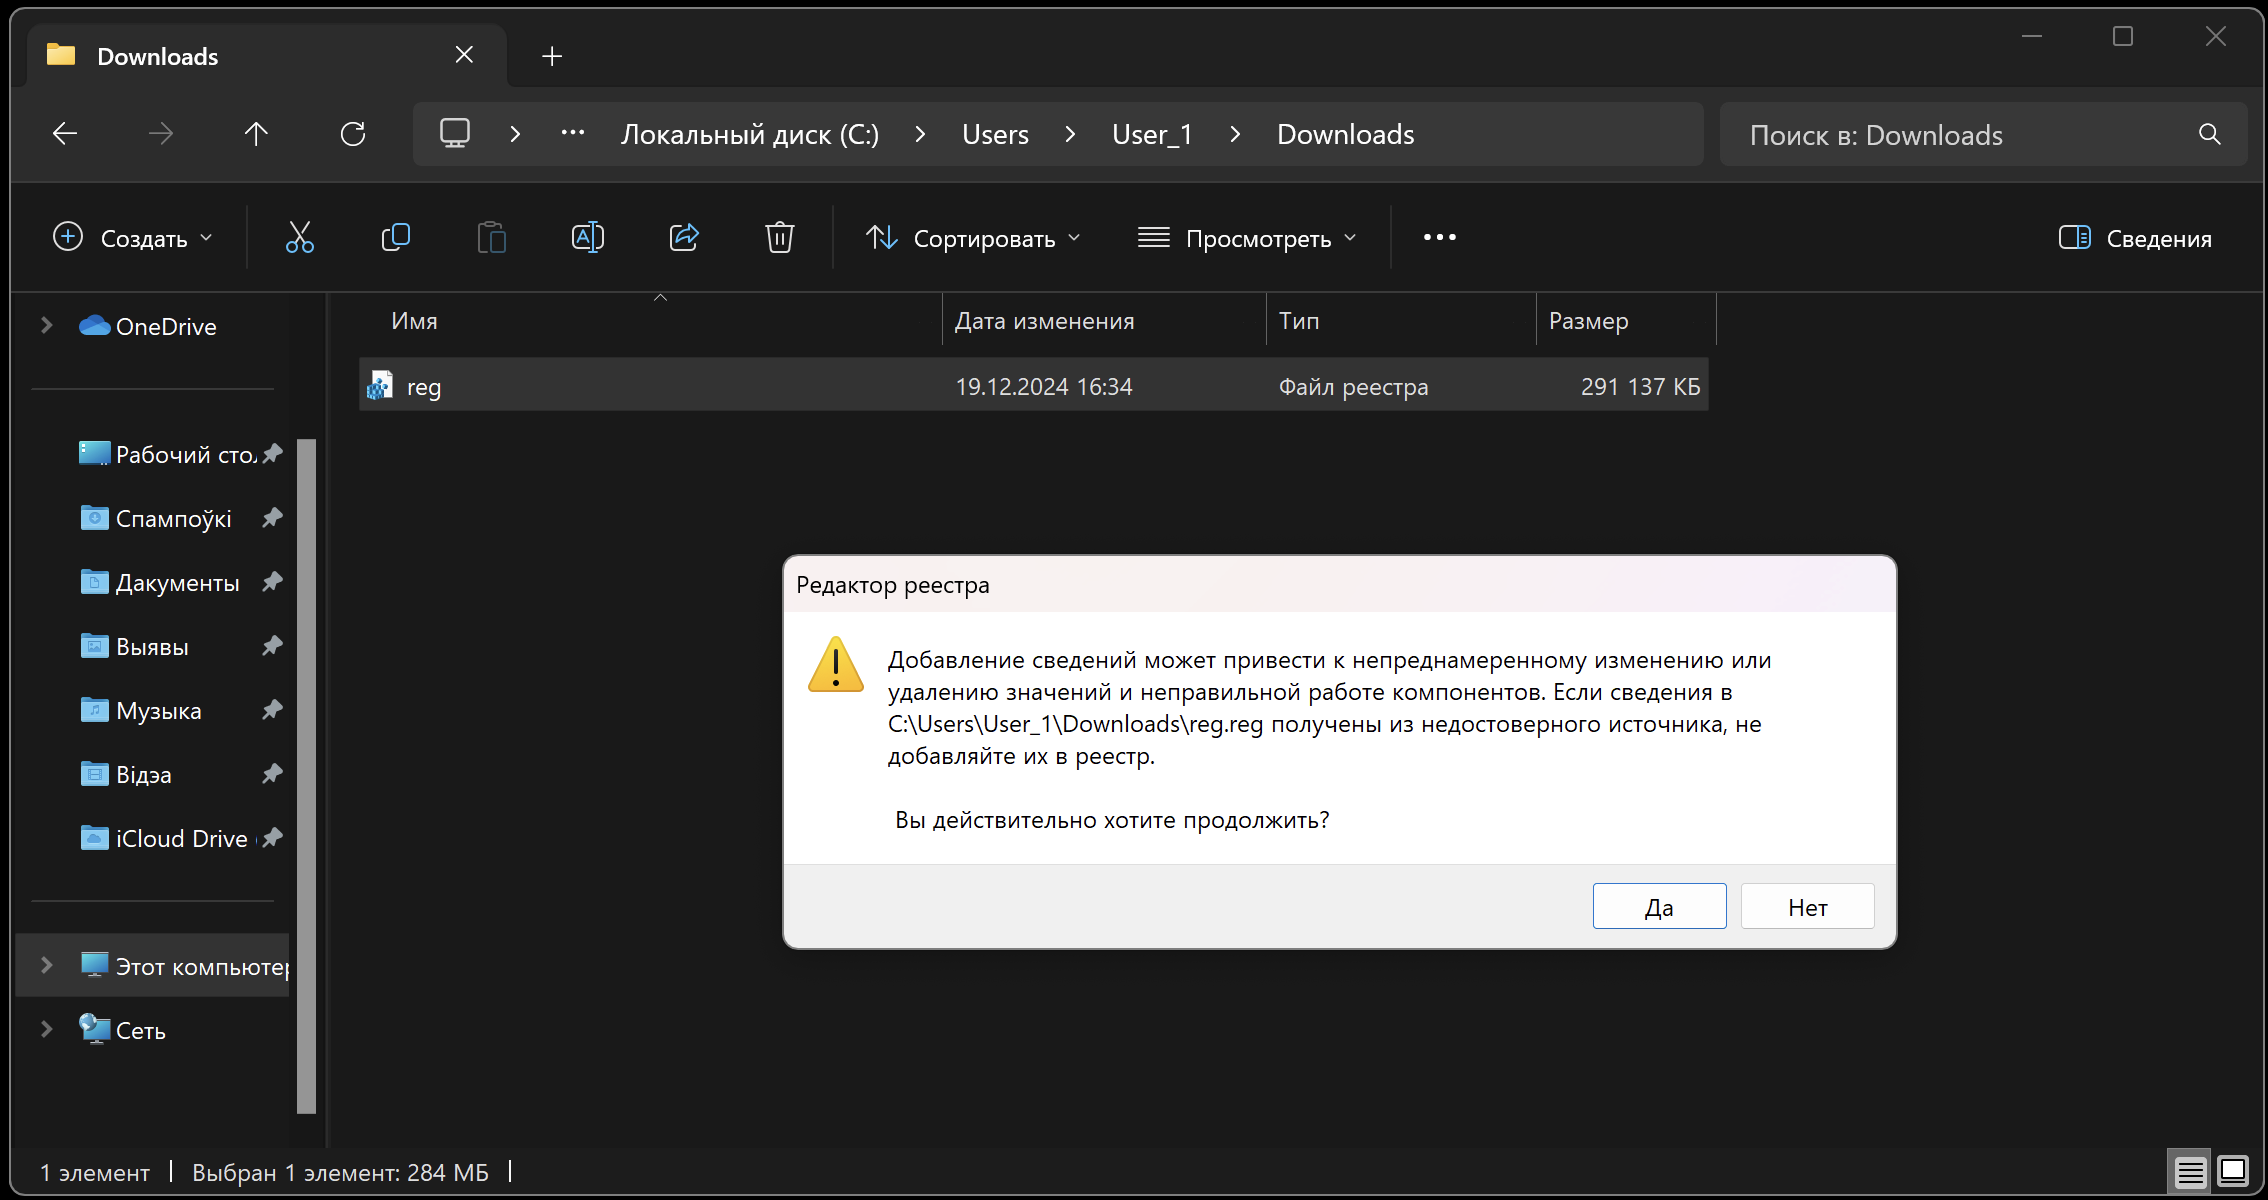
\includegraphics[width=0.8\textwidth]{../images/regedit_import.png}
                                  \caption{Восстановление реестра}
                              \end{figure}
                              }
                    \end{enumerate}
                    }
          \end{enumerate}
          }
    \item {\textbf{Использование утилиты SFC}

          Утилита SFC (System File Checker) позволяет восстановить поврежденные системные файлы, включая файлы реестра.

          \textbf{Шаги:}
          \begin{enumerate}
              \item Откройте командную строку с правами администратора.
              \item {Введите команду:
                    \begin{lstlisting}[language=bash]
sfc /scannow
                            \end{lstlisting}
                    }
              \item Подождите, пока система проверит и восстановит поврежденные файлы.

                    \begin{figure}[H]
                        \centering
                        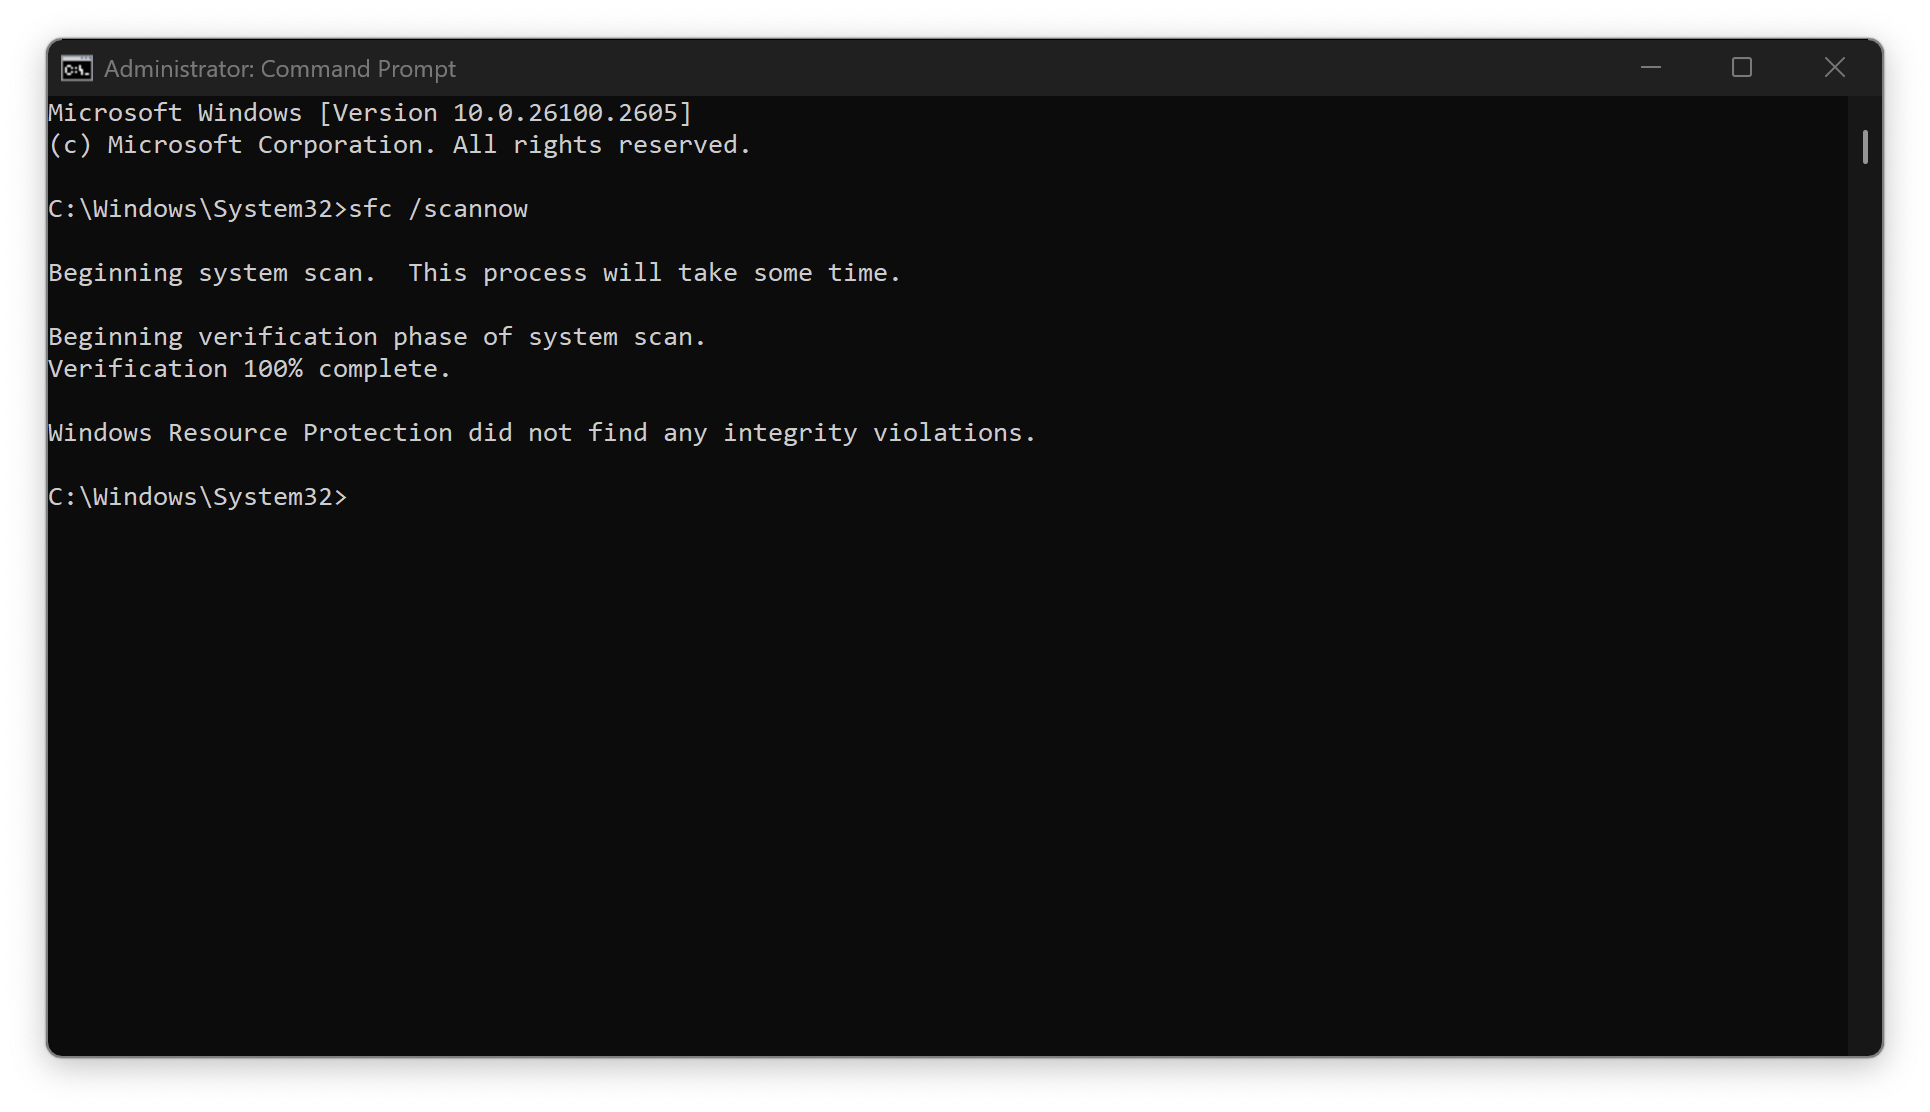
\includegraphics[width=0.8\textwidth]{../images/sfc.png}
                        \caption{Использование утилиты SFC}
                    \end{figure}
          \end{enumerate}
          }
    \item {\textbf{Восстановление через точки восстановления}

          Точки восстановления создаются системой автоматически или вручную и содержат резервные копии системных файлов, включая реестр.

          \textbf{Примечание:} Функция точек восстановления может быть отключена по умолчанию.

          \textbf{Шаги:}
          \begin{enumerate}
              \item {Откройте \verb|Свойства системы|, выберите \verb|Настройка параметров восстановления|.
                    \begin{figure}[H]
                        \centering
                        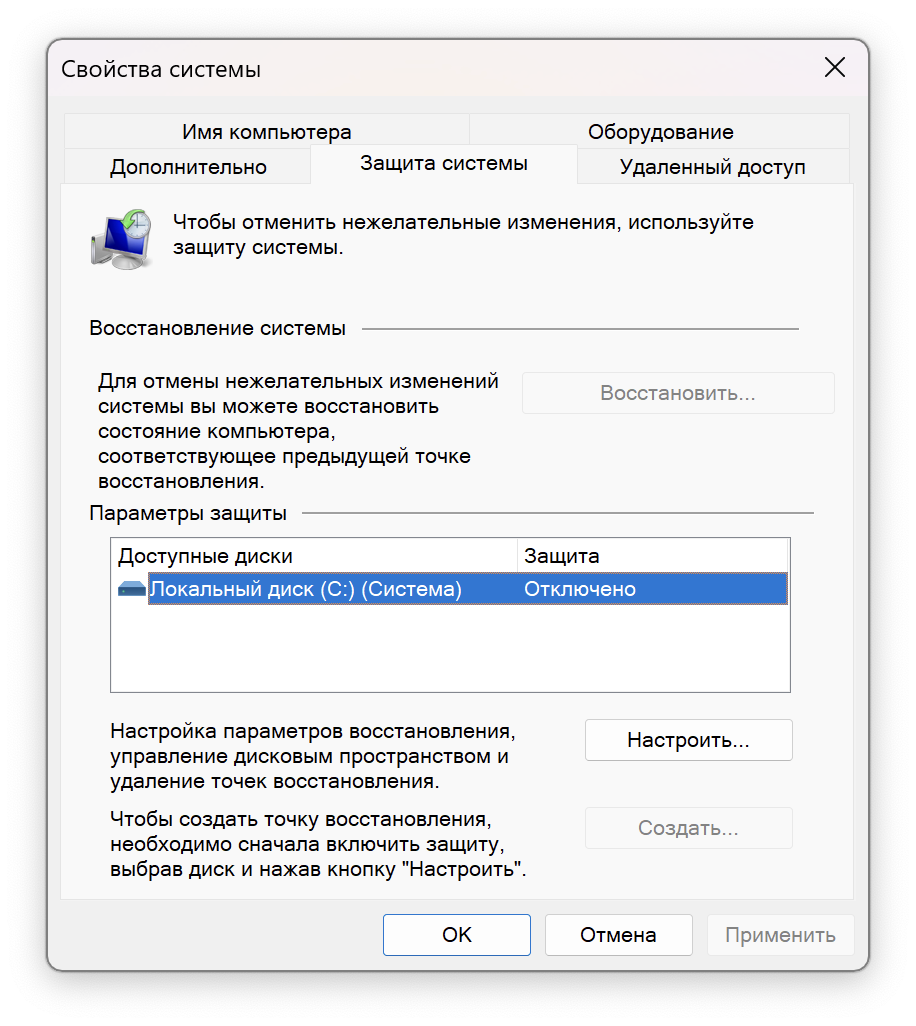
\includegraphics[width=0.5\textwidth]{../images/properties-of-system.png}
                        \caption{Свойства системы}
                    \end{figure}
                    }
              \item {Включите защиту системы.
                    \begin{figure}[H]
                        \centering
                        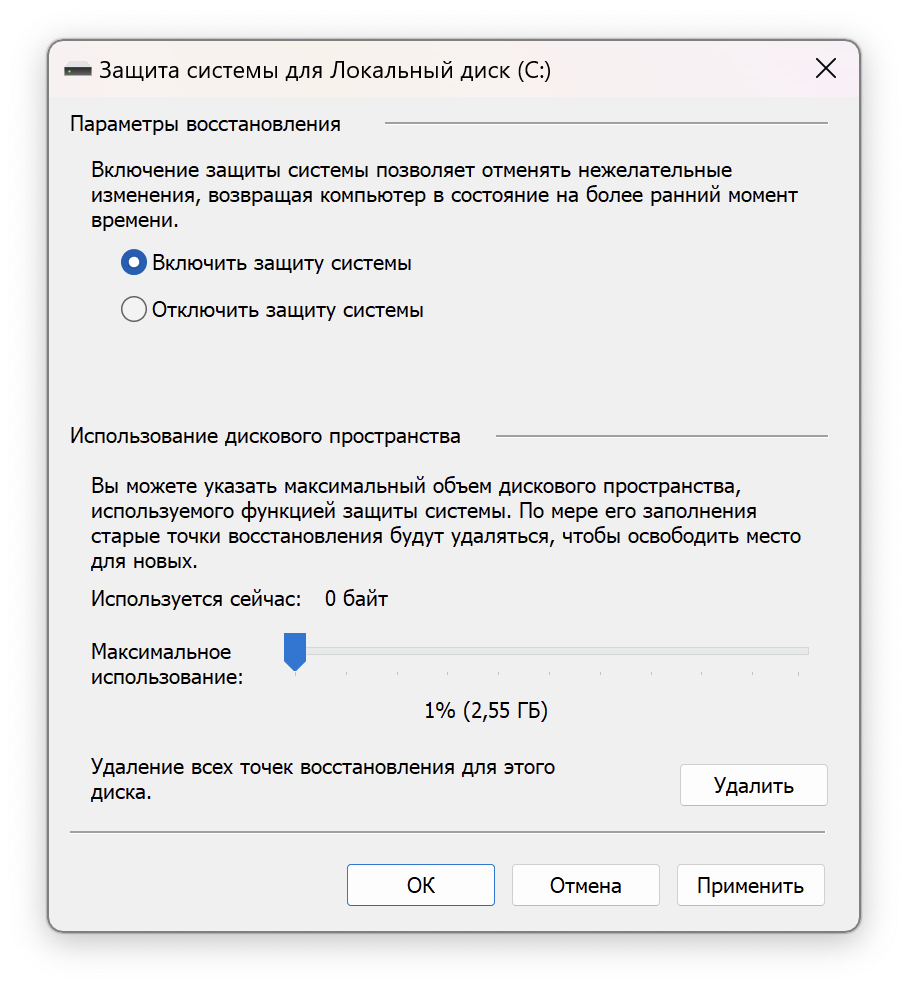
\includegraphics[width=0.5\textwidth]{../images/enable-system-restore.png}
                        \caption{Включение защиты системы}
                    \end{figure}
                    }
              \item {Нажмите на «Создать точку восстановления для дисков с включенной функцией защиты системы.»}
              \item {Создайте точку восстановления.
                    \begin{figure}[H]
                        \centering
                        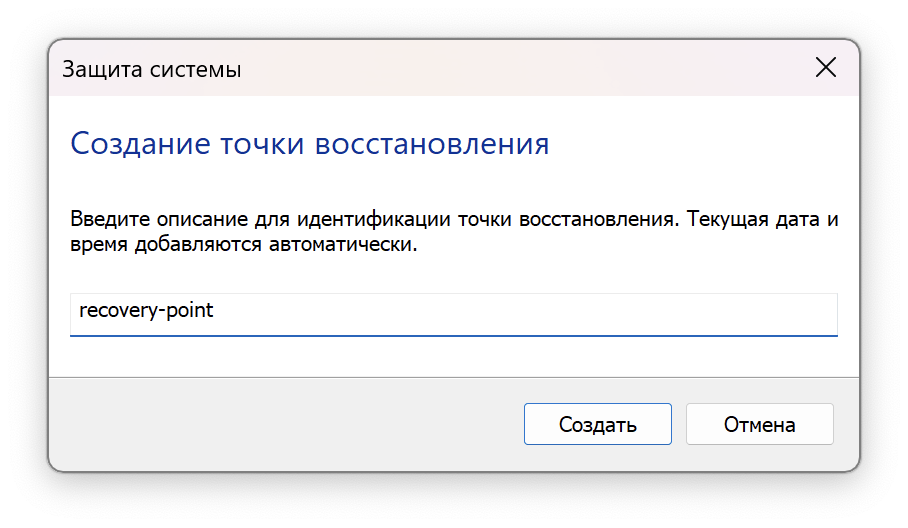
\includegraphics[width=0.8\textwidth]{../images/create-restore-point.png}
                        \caption{Создание точки восстановления}
                    \end{figure}
                    }
              \item {После успешного создания точки восстановления, появится кнопка \verb|Восстановить|. Нажмите на нее и выберите точку восстановления.
                    \begin{figure}[H]
                        \centering
                        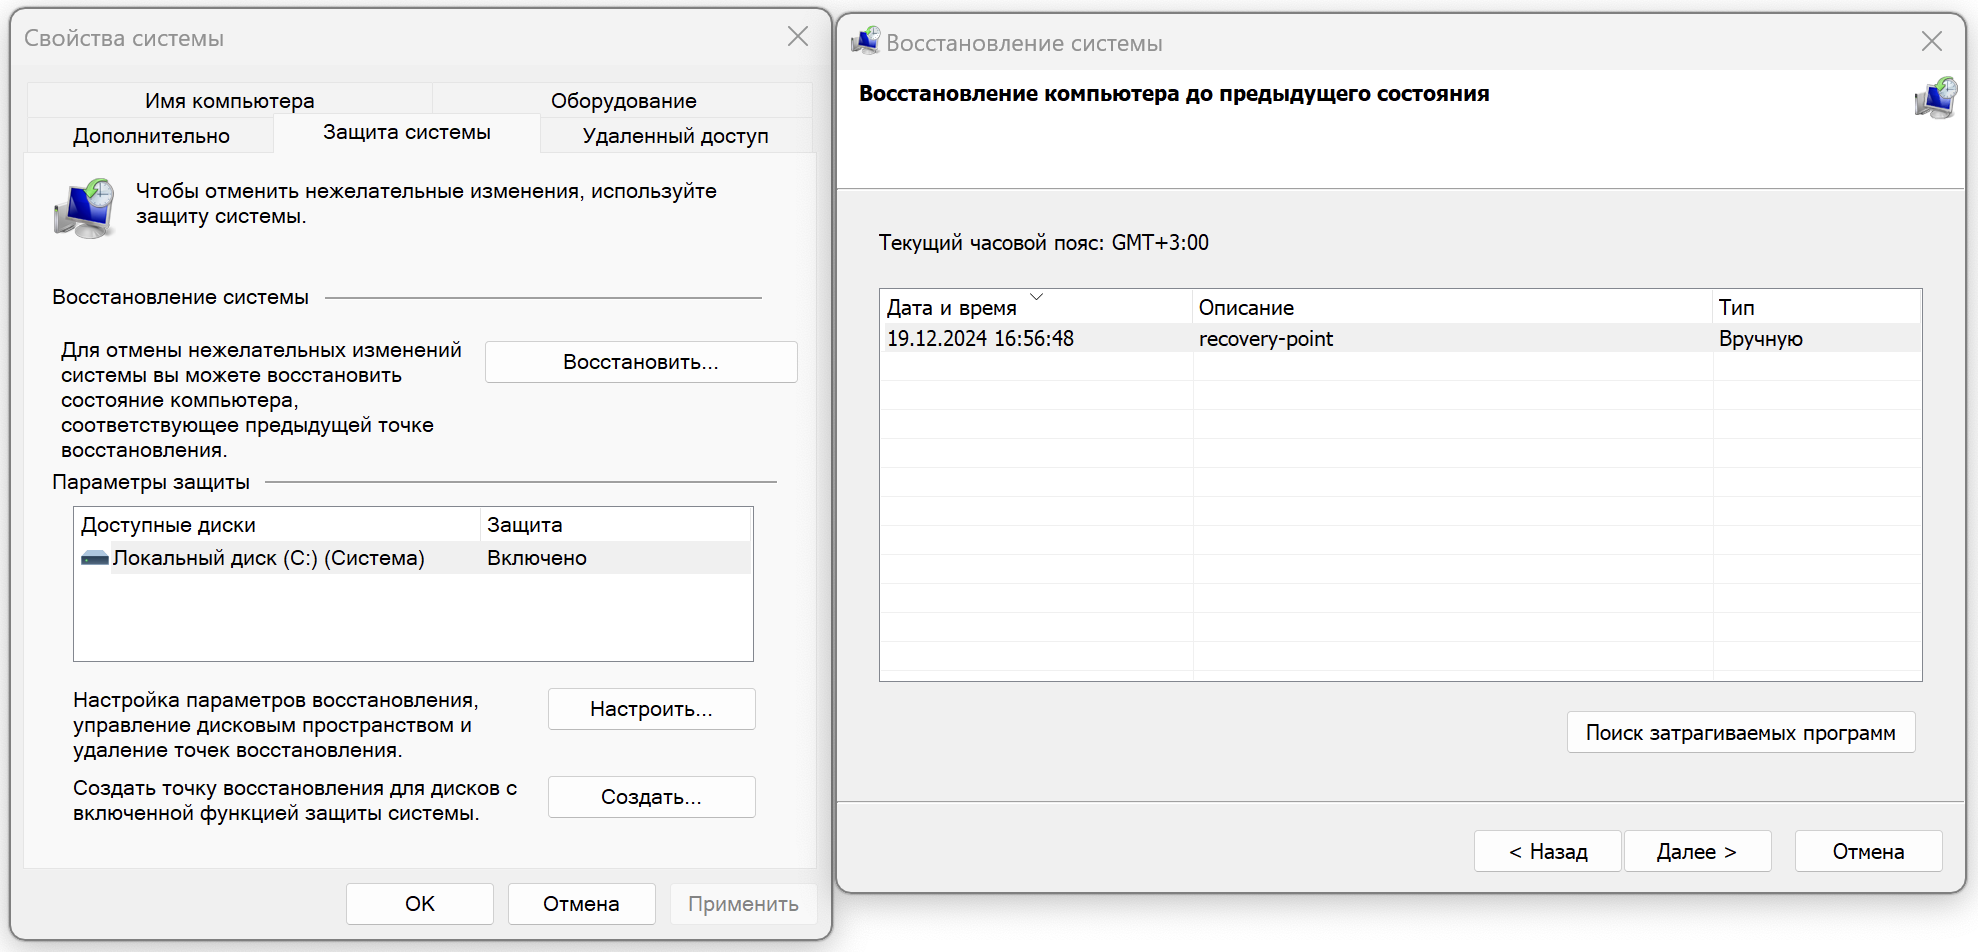
\includegraphics[width=0.8\textwidth]{../images/restore-system.png}
                        \caption{Восстановление системы}
                    \end{figure}}
              \item {Подтвердите точку восстановления.
                    \begin{figure}[H]
                        \centering
                        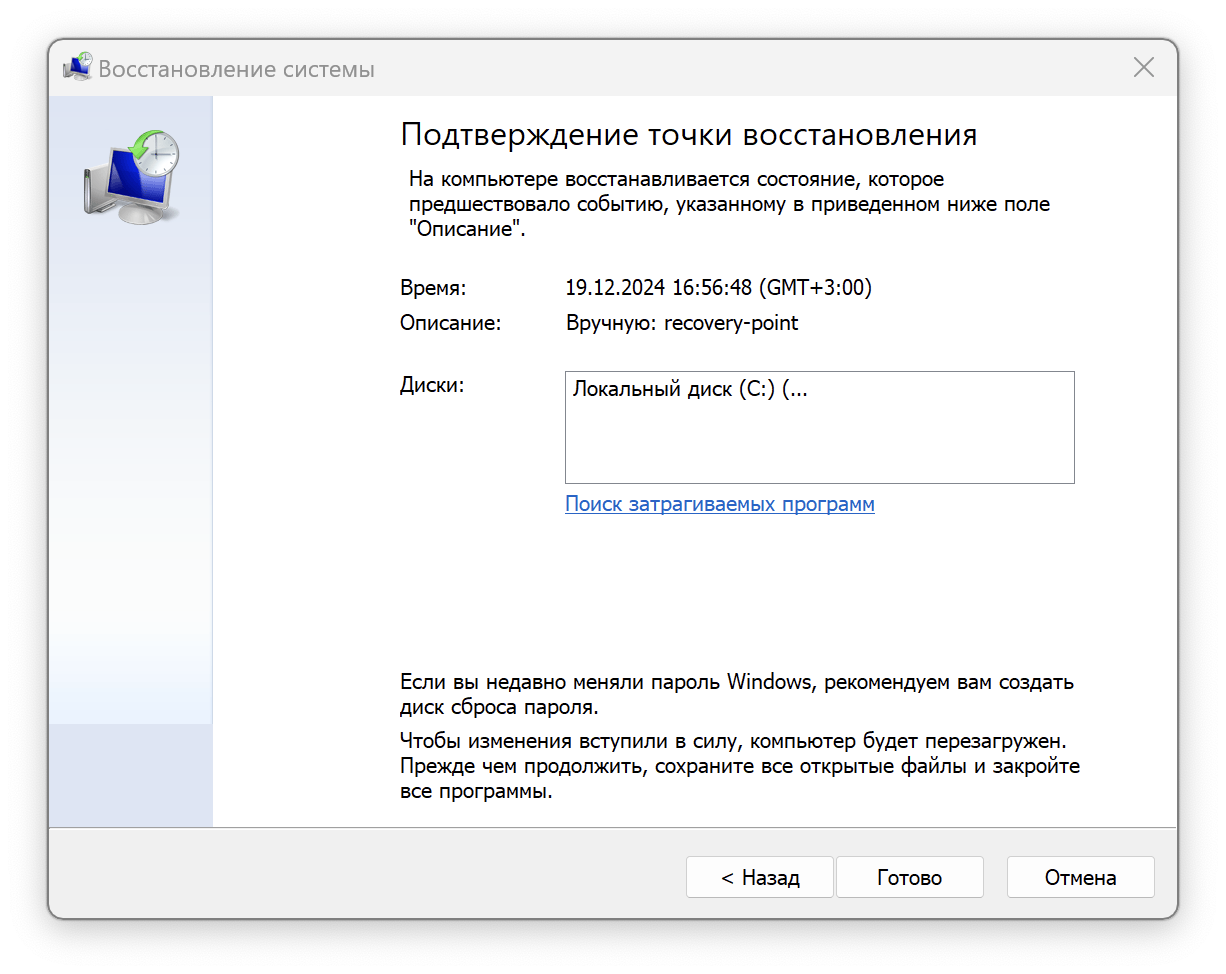
\includegraphics[width=0.8\textwidth]{../images/restore-system-confirmation.png}
                        \caption{Подтверждение точки восстановления}
                    \end{figure}
                    }
          \end{enumerate}
          }
    \item{\textbf{Восстановление через сброс системы}

          Если другие методы не помогли, можно воспользоваться сбросом системы.

          \textbf{Шаги:}
          \begin{enumerate}
              \item В «Параметры» откройте раздел «Система» $\rightarrow$ «Восстановление». Выберите пункт «Вернуть компьютер в исходное состояние».
              \item Выберите опцию «Сохранить мои файлы» или «Удалить всё».
              \item Следуйте инструкциям на экране.
          \end{enumerate}
          \begin{figure}[H]
              \centering
              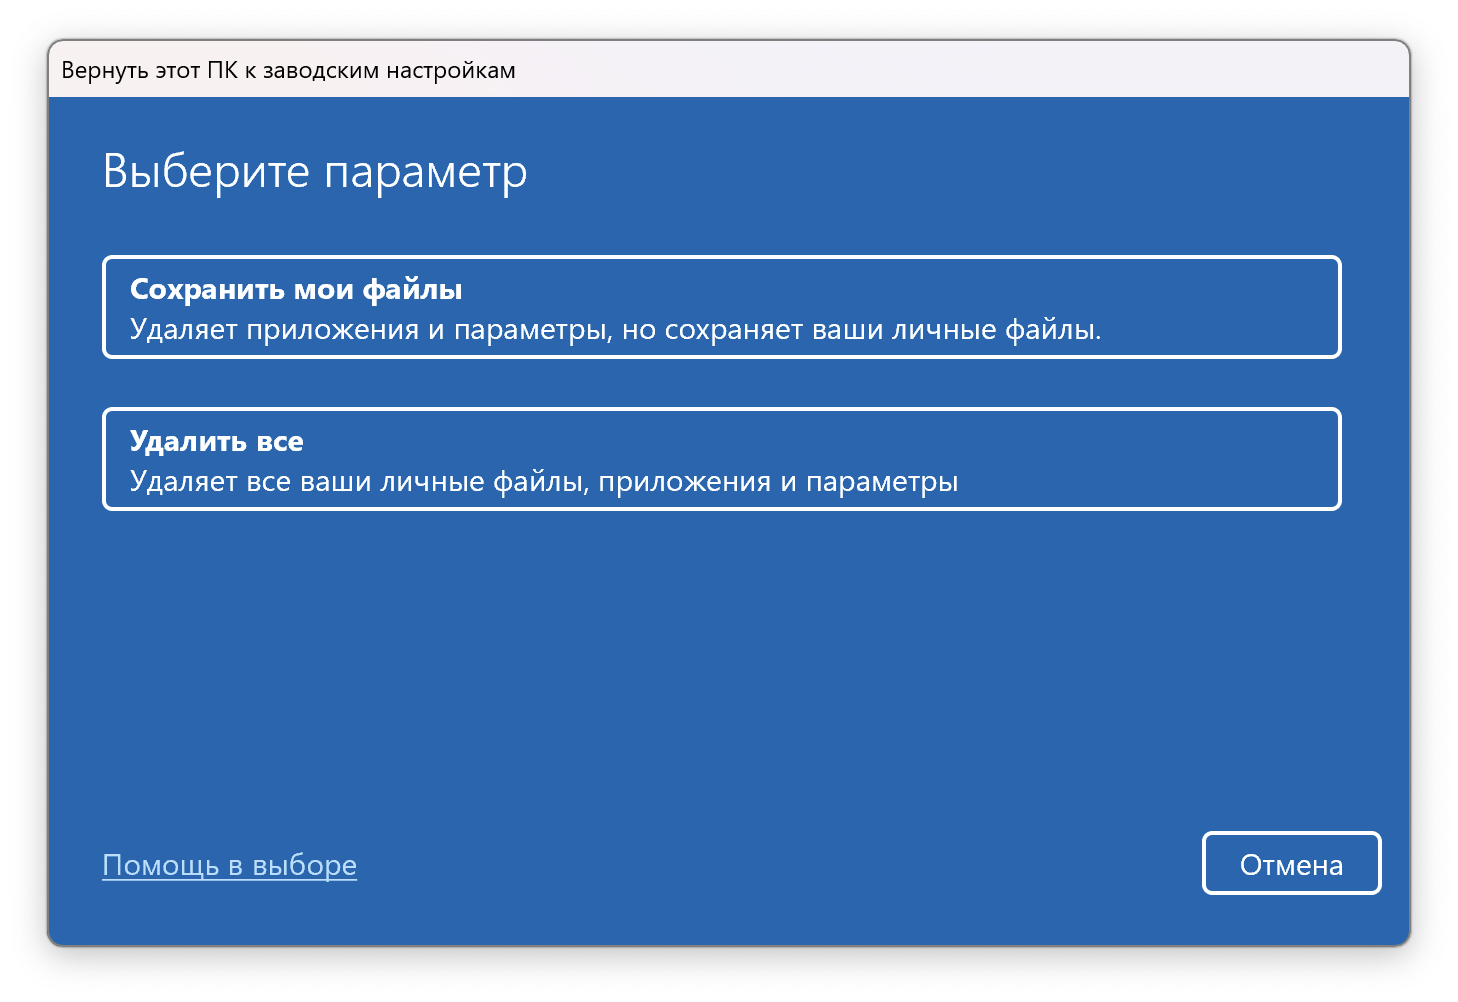
\includegraphics[width=0.8\textwidth]{../images/reset-system.png}
              \caption{Восстановление через сброс системы}
          \end{figure}
          \textbf{Примечание:}  Этот метод удаляет все пользовательские программы и настройки, но сохраняет личные файлы.
          }
\end{enumerate}
\section{Настройка службы Superfetch: включение механизма Prefetcher только для загрузки системы.}

Superfetch анализирует ваш рабочий процесс и предзагружает часто используемые приложения и данные в оперативную память, чтобы ускорить доступ к ним.

Однако, на современных компьютерах данная функция не особо нужна, более того, для твердотельных дисков SSD SuperFetch и PreFetch рекомендуется отключить.

\textbf{Шаги для настройки Prefetcher только для загрузки системы:}
\begin{enumerate}
    \item {Откройте редактор реестра:
    \item Нажмите \verb|Win + R|, чтобы открыть окно «Выполнить».
    \item Введите \verb|regedit| и нажмите \verb|Enter|.
          }
    \item {Перейдите к ключу реестра:
          \begin{itemize}
              \item \verb|HKEY_LOCAL_MACHINE\|
                    \verb|SYSTEM\|
                    \verb|CurrentControlSet\|
                    \verb|Control\|
                    \verb|Session Manager\|
                    \verb|Memory Management\|
                    \verb|PrefetchParameters|
          \end{itemize}}
    \item {Найдите параметр EnablePrefetcher:
          \begin{itemize}
              \item В правой части окна найдите параметр \verb|EnablePrefetcher|.
              \item {Если его нет, создайте его:
                    \begin{enumerate}
                        \item Щелкните правой кнопкой мыши на пустом пространстве в правой части окна.
                        \item Выберите \verb|Создать| > \verb|DWORD (32-разрядный) значение|.
                        \item Назовите его \verb|EnablePrefetcher|.
                    \end{enumerate}}
          \end{itemize}
          }
    \item {Измените значение \verb|EnablePrefetcher|:
          \begin{itemize}
              \item Дважды щелкните на \verb|EnablePrefetcher|.
              \item {Установите значение в зависимости от ваших потребностей:
                    \begin{itemize}
                        \item \verb|0| - Prefetcher отключен.
                        \item \verb|1| - Prefetcher включен только для загрузки системы.
                        \item \verb|2| - Prefetcher включен только для загрузки приложений.
                        \item \verb|3| - Prefetcher включен для загрузки системы и приложений (режим по умолчанию).
                    \end{itemize}}
              \item \textbf{Примечание:} Для редактирования реестра необходимо иметь права администратора.
              \item {Для нашего случая необходимо установить значение \verb|1|.
                    \begin{figure}[H]
                        \centering
                        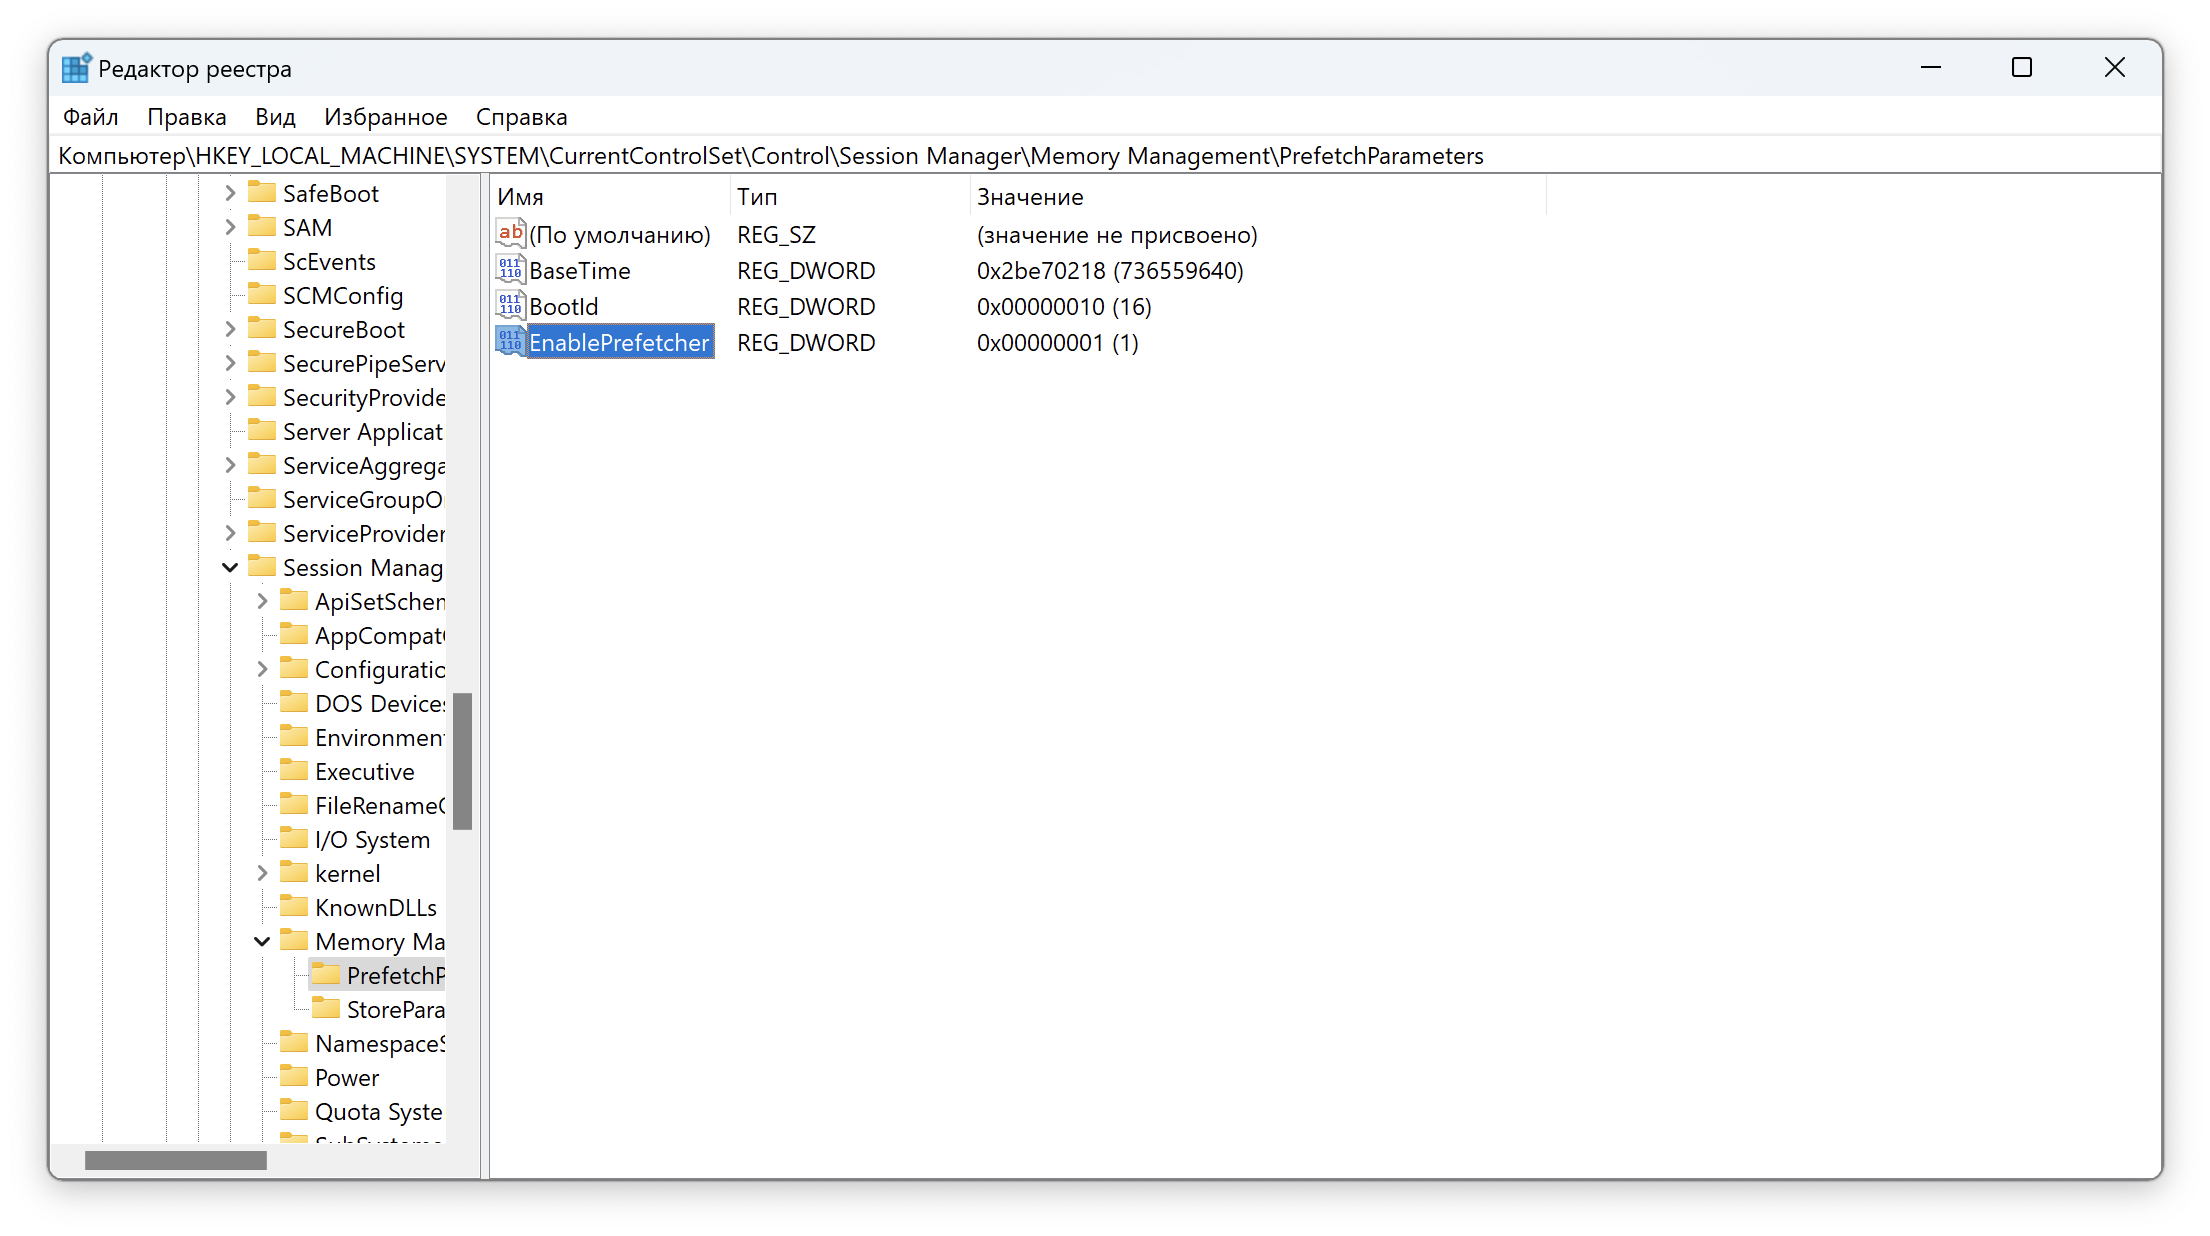
\includegraphics[width=0.8\textwidth]{../images/regedit_prefetcher.png}
                        \caption{Настройка Prefetcher}
                    \end{figure}
                    }
          \end{itemize}
          }
    \item {Примените изменения:
          \begin{itemize}
              \item Нажмите \verb|OK|, чтобы сохранить изменения.
              \item Закройте редактор реестра.
          \end{itemize}
          }
    \item {Перезагрузите систему:
          \begin{itemize}
              \item Перезагрузите компьютер, чтобы изменения вступили в силу.
          \end{itemize}}
\end{enumerate}
\section{Увеличение скорости выключения компьютера.}
\textbf{Шаги для увеличения скорости выключения:}
\begin{enumerate}
    \item {Откройте Редактор реестра:
          \begin{itemize}
              \item \verb|Win + R|, чтобы открыть окно «Выполнить».
              \item Введите \verb|regedit| и нажмите \verb|Enter|.
          \end{itemize}
          }
    \item {Перейдите к нужному разделу реестра:
          \begin{itemize}
              \item В редакторе реестра перейдите по следующему пути:\\ \verb|HKEY_LOCAL_MACHINE\|
                    \verb|SYSTEM\|
                    \verb|CurrentControlSet\|
                    \verb|Control|
          \end{itemize}
          }
    \item {Найдите параметр «WaitToKillServiceTimeout»:
          \begin{itemize}
              \item В правой части окна найдите параметр с именем \verb|WaitToKillServiceTimeout|.
              \item {Если этого параметра нет, вы можете создать его:
                    \begin{enumerate}
                        \item Щелкните правой кнопкой мыши на пустом пространстве в правой части окна.
                        \item Выберите \verb|Создать| > \verb|Строковое значение|.
                        \item Назовите его \verb|WaitToKillServiceTimeout|.
                    \end{enumerate}
                    }
          \end{itemize}
          }
    \item {Измените значение параметра:
          \begin{itemize}
              \item Дважды щелкните на \verb|WaitToKillServiceTimeout|.
              \item По умолчанию значение может быть установлено на \verb|5000| (5 секунд). Вы можете уменьшить это значение, например, до \verb|1000| (1 секунды).
              \item Введите новое значение и нажмите \verb|ОК|.
                    {\begin{figure}[H]
                        \centering
                        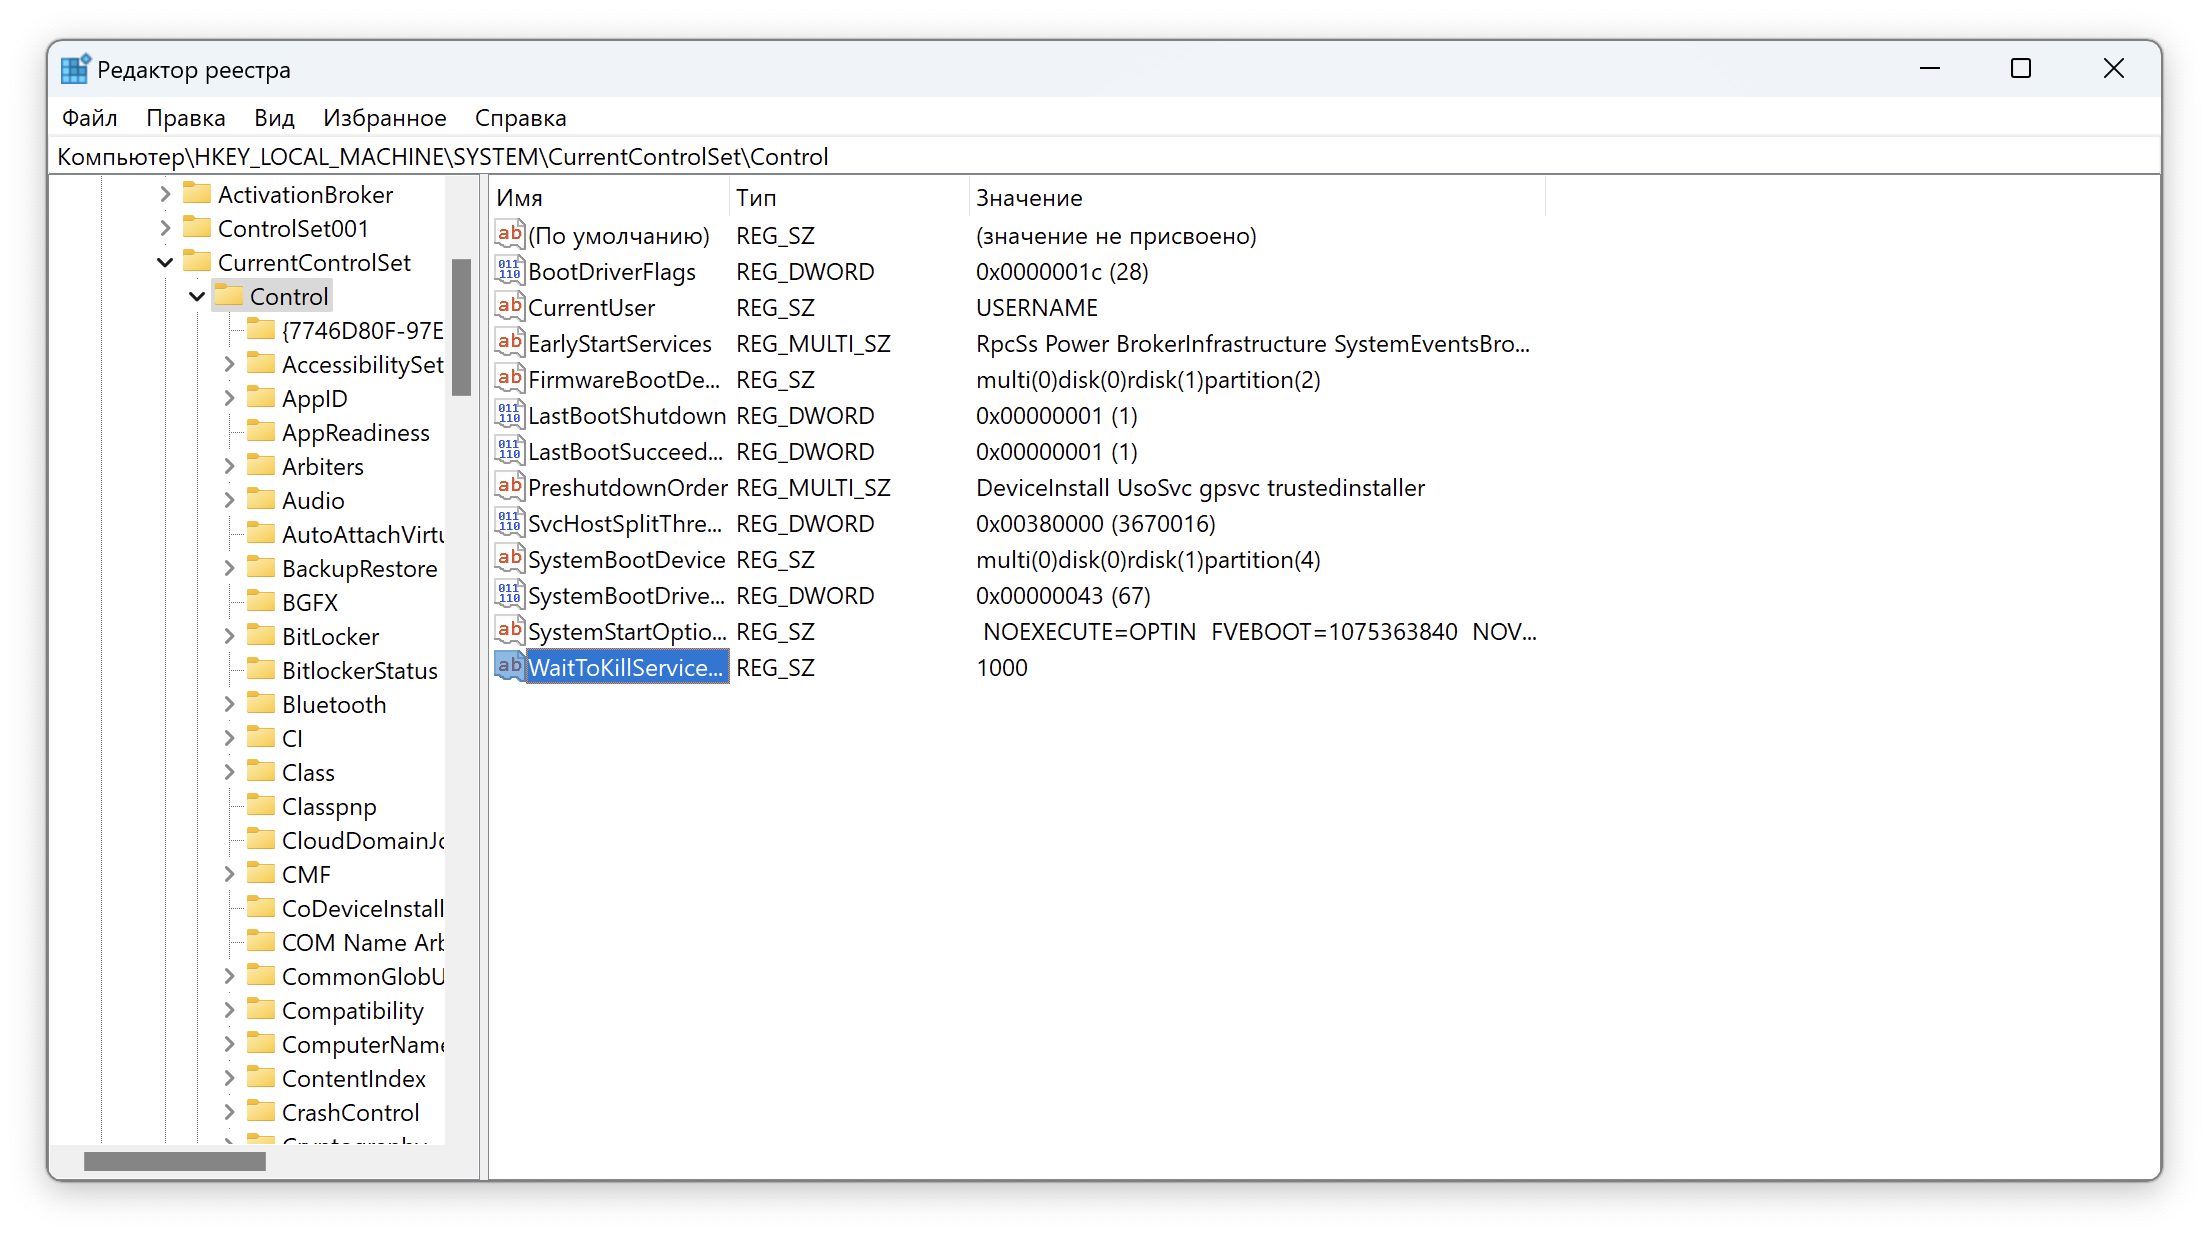
\includegraphics[width=0.8\textwidth]{../images/regedit_wait_to_kill_service_timeout.png}
                        \caption{Настройка скорости выключения}
                    \end{figure}}
              \item \textbf{Примечание:} Для редактирования реестра необходимо иметь права администратора.
          \end{itemize}
          }
    \item {Также ускорить выключение можно, выключив отчиску файла подкачки.
          \begin{itemize}
              \item Перейдите к ключу реестра:
                    \begin{itemize}
                        \item \verb|HKEY_LOCAL_MACHINE\|
                              \verb|SYSTEM\|
                              \verb|CurrentControlSet\|
                              \verb|Control\|
                              \verb|Session Manager\|
                              \verb|Memory Management|
                    \end{itemize}
              \item {Найдите параметр \verb|ClearPageFileAtShutdown|.
                    \begin{itemize}
                        \item В правой части окна находится параметр \verb|ClearPageFileAtShutdown|.
                        \item {Если его нет, создайте его:
                              \begin{enumerate}
                                  \item Щелкните правой кнопкой мыши на пустом пространстве в правой части окна.
                                  \item Выберите \verb|Создать| > \verb|DWORD (32-разрядный) значение|.
                                  \item Назовите его \verb|ClearPageFileAtShutdown|.
                              \end{enumerate}}
                    \end{itemize}
                    }
              \item {Измените значение \verb|ClearPageFileAtShutdown|:
                    \begin{itemize}
                        \item Дважды щелкните на \verb|ClearPageFileAtShutdown|.
                        \item Установите значение в \verb|0|.
                              \begin{figure}[H]
                                  \centering
                                  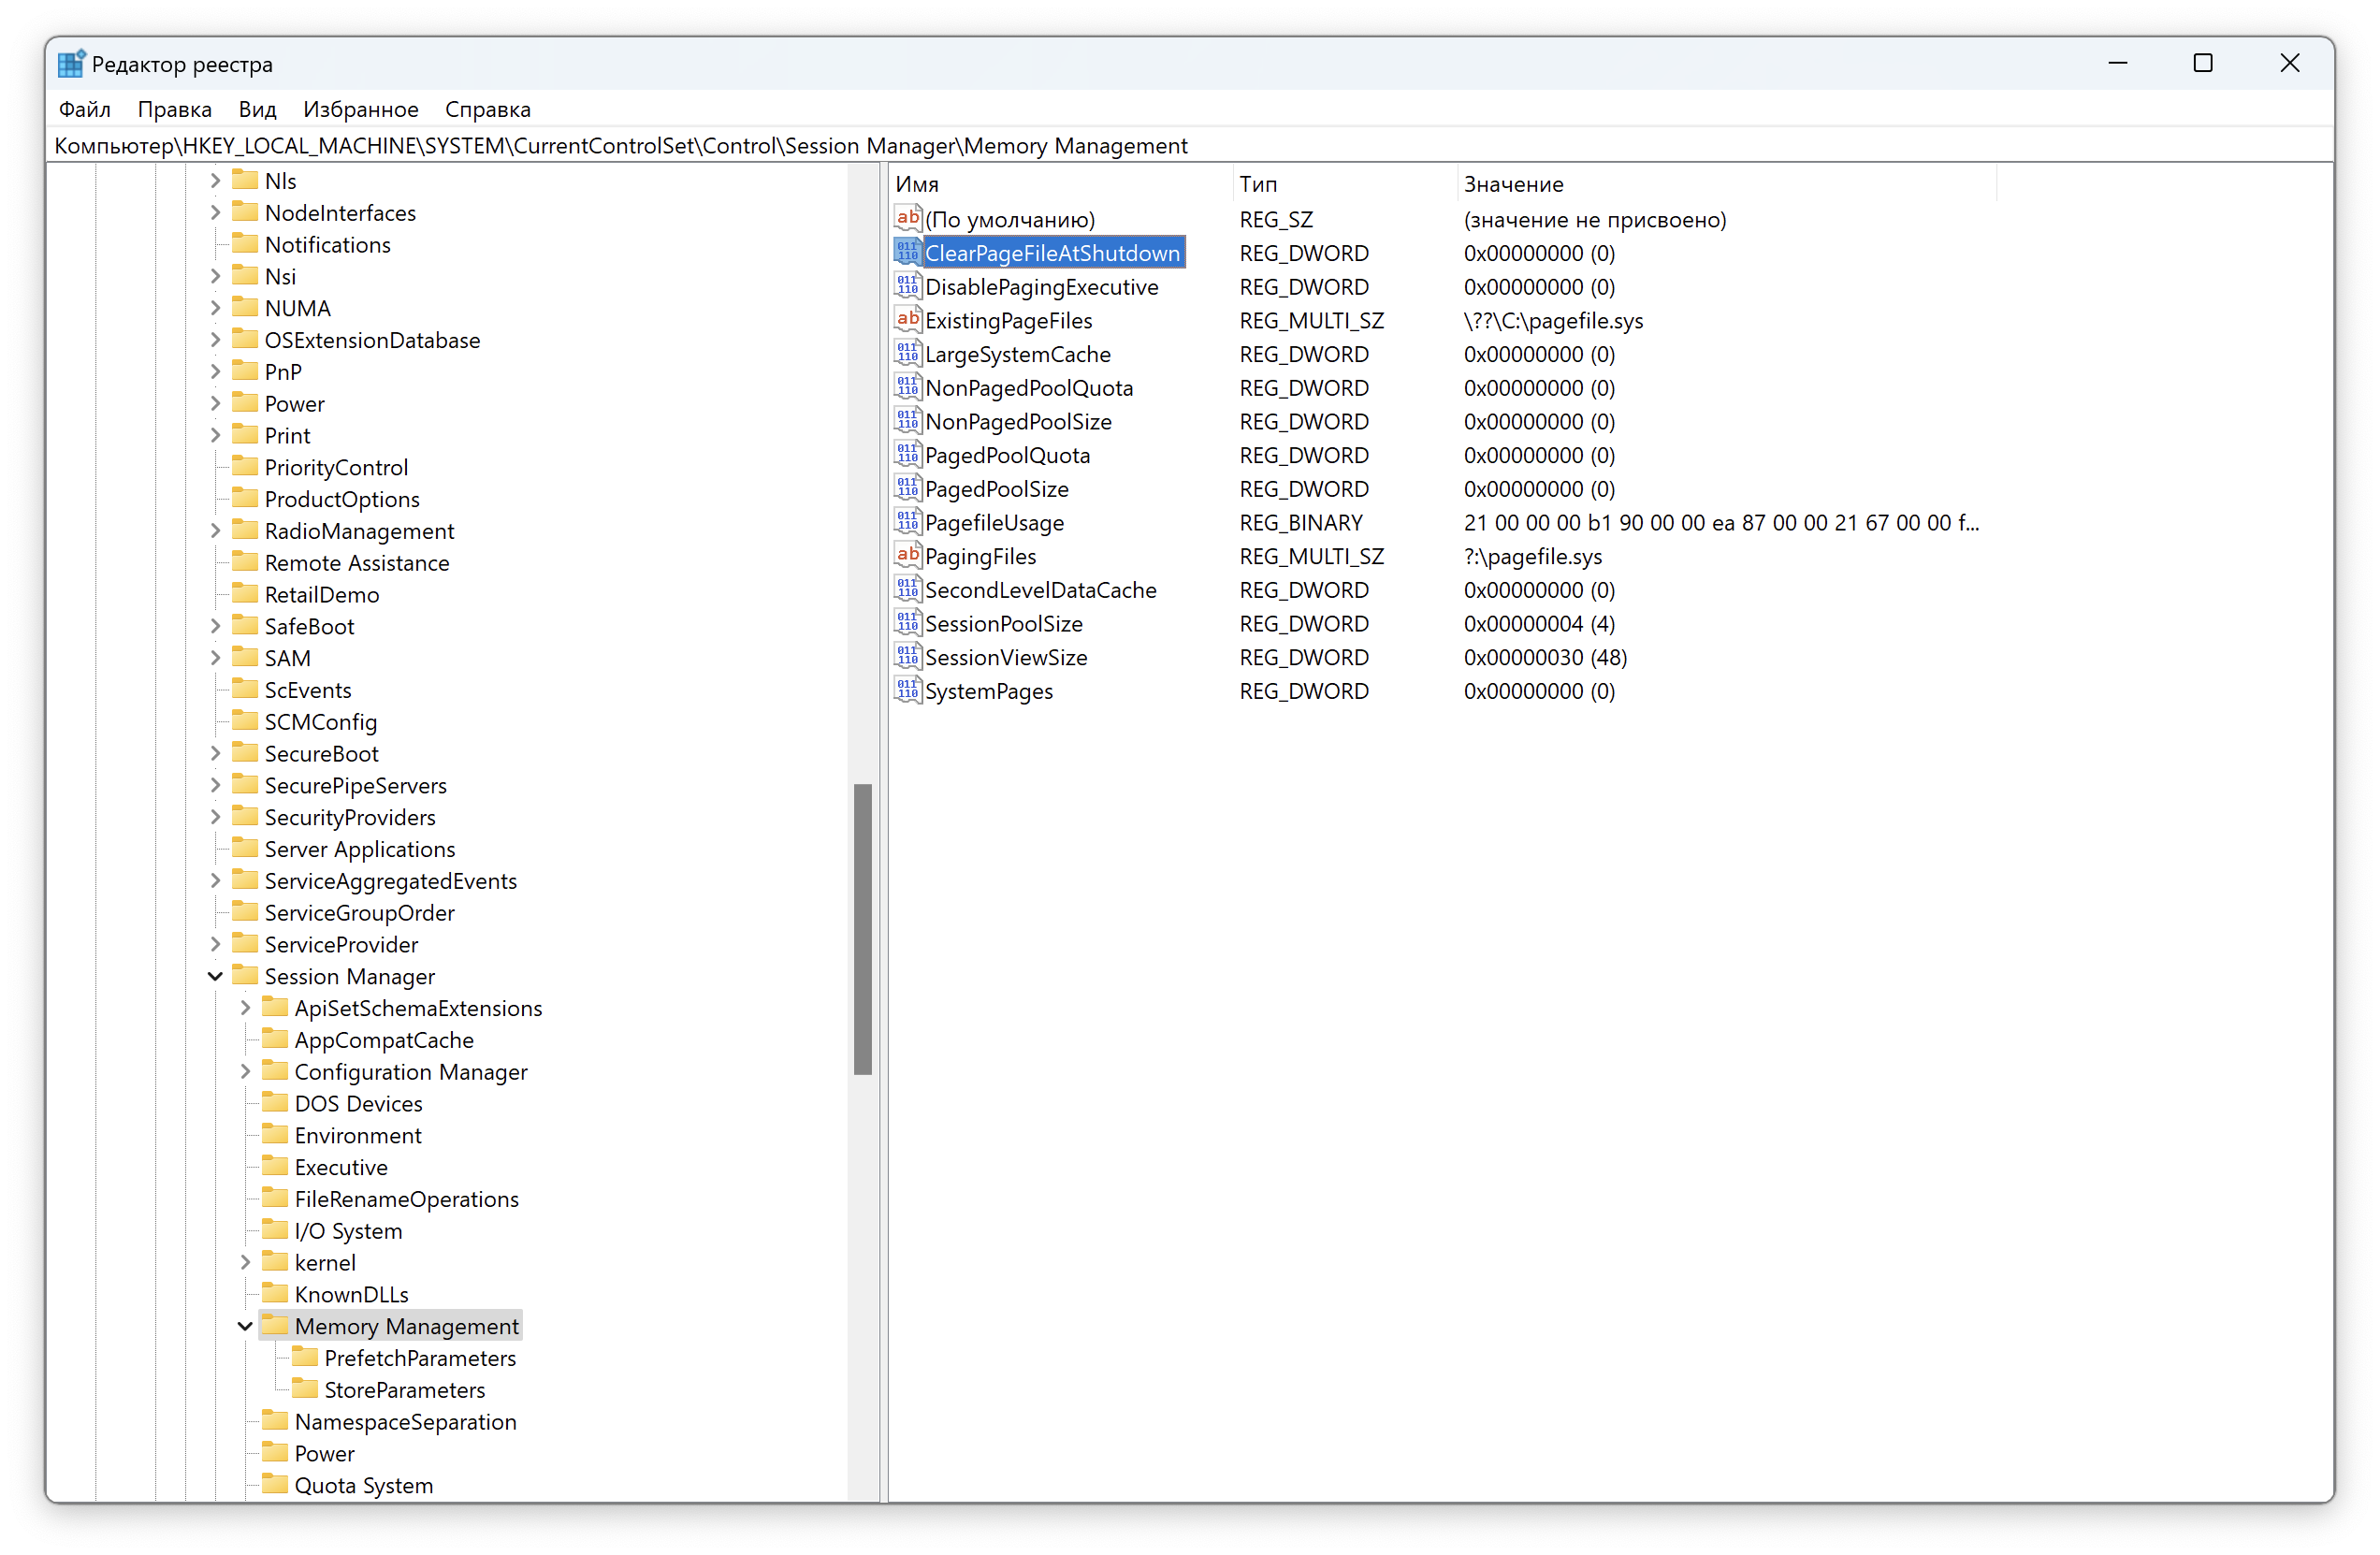
\includegraphics[width=0.8\textwidth]{../images/regedit_clear_page_file_at_shutdown.png}
                                  \caption{Настройка скорости выключения}
                              \end{figure}
                        \item \textbf{Примечание:} Для редактирования реестра необходимо иметь права администратора.
                    \end{itemize}
                    }
          \end{itemize}
          }
    \item {Перезагрузите компьютер:
          \begin{itemize}
              \item После внесения изменений перезагрузите компьютер, чтобы изменения вступили в силу.
          \end{itemize}}
\end{enumerate}
\section{Деактивация клавиши Win.}
\textbf{Шаги для деактивации клавиши Win через реестр:}
\begin{enumerate}
    \item {Откройте Редактор реестра:
          \begin{itemize}
              \item \verb|Win + R|, чтобы открыть окно «Выполнить».
              \item Введите \verb|regedit| и нажмите \verb|Enter|.
          \end{itemize}
          }
    \item {Перейдите к нужному разделу реестра:
          \begin{itemize}
              \item В редакторе реестра перейдите по следующему пути:\\
                    \verb|HKEY_LOCAL_MACHINE\|
                    \verb|SYSTEM\|
                    \verb|CurrentControlSet\|
                    \verb|Control\|
                    \verb|Keyboard Layout|
          \end{itemize}
          }
    \item {Создать новый бинарный ключ:
          \begin{itemize}
              \item В правой части окна найдите пустое пространство и щелкните правой кнопкой мыши.
              \item Выберите \verb|Создать| > \verb|Двоичное значение|.
              \item Назовите его \verb|Scancode Map|.
          \end{itemize}
          }
    \item {Изменить значение ключа:
          \begin{itemize}
              \item Дважды щелкните на созданном ключе \verb|Scancode Map|.
              \item {Введите следующее значение:
                    \begin{lstlisting}
00 00 00 00 00 00 00 00
03 00 00 00 00 00 5B E0
00 00 5C E0 00 00 00 00
                    \end{lstlisting}}
              \item Это значение отключает клавишу Win.
                    \begin{figure}[H]
                        \centering
                        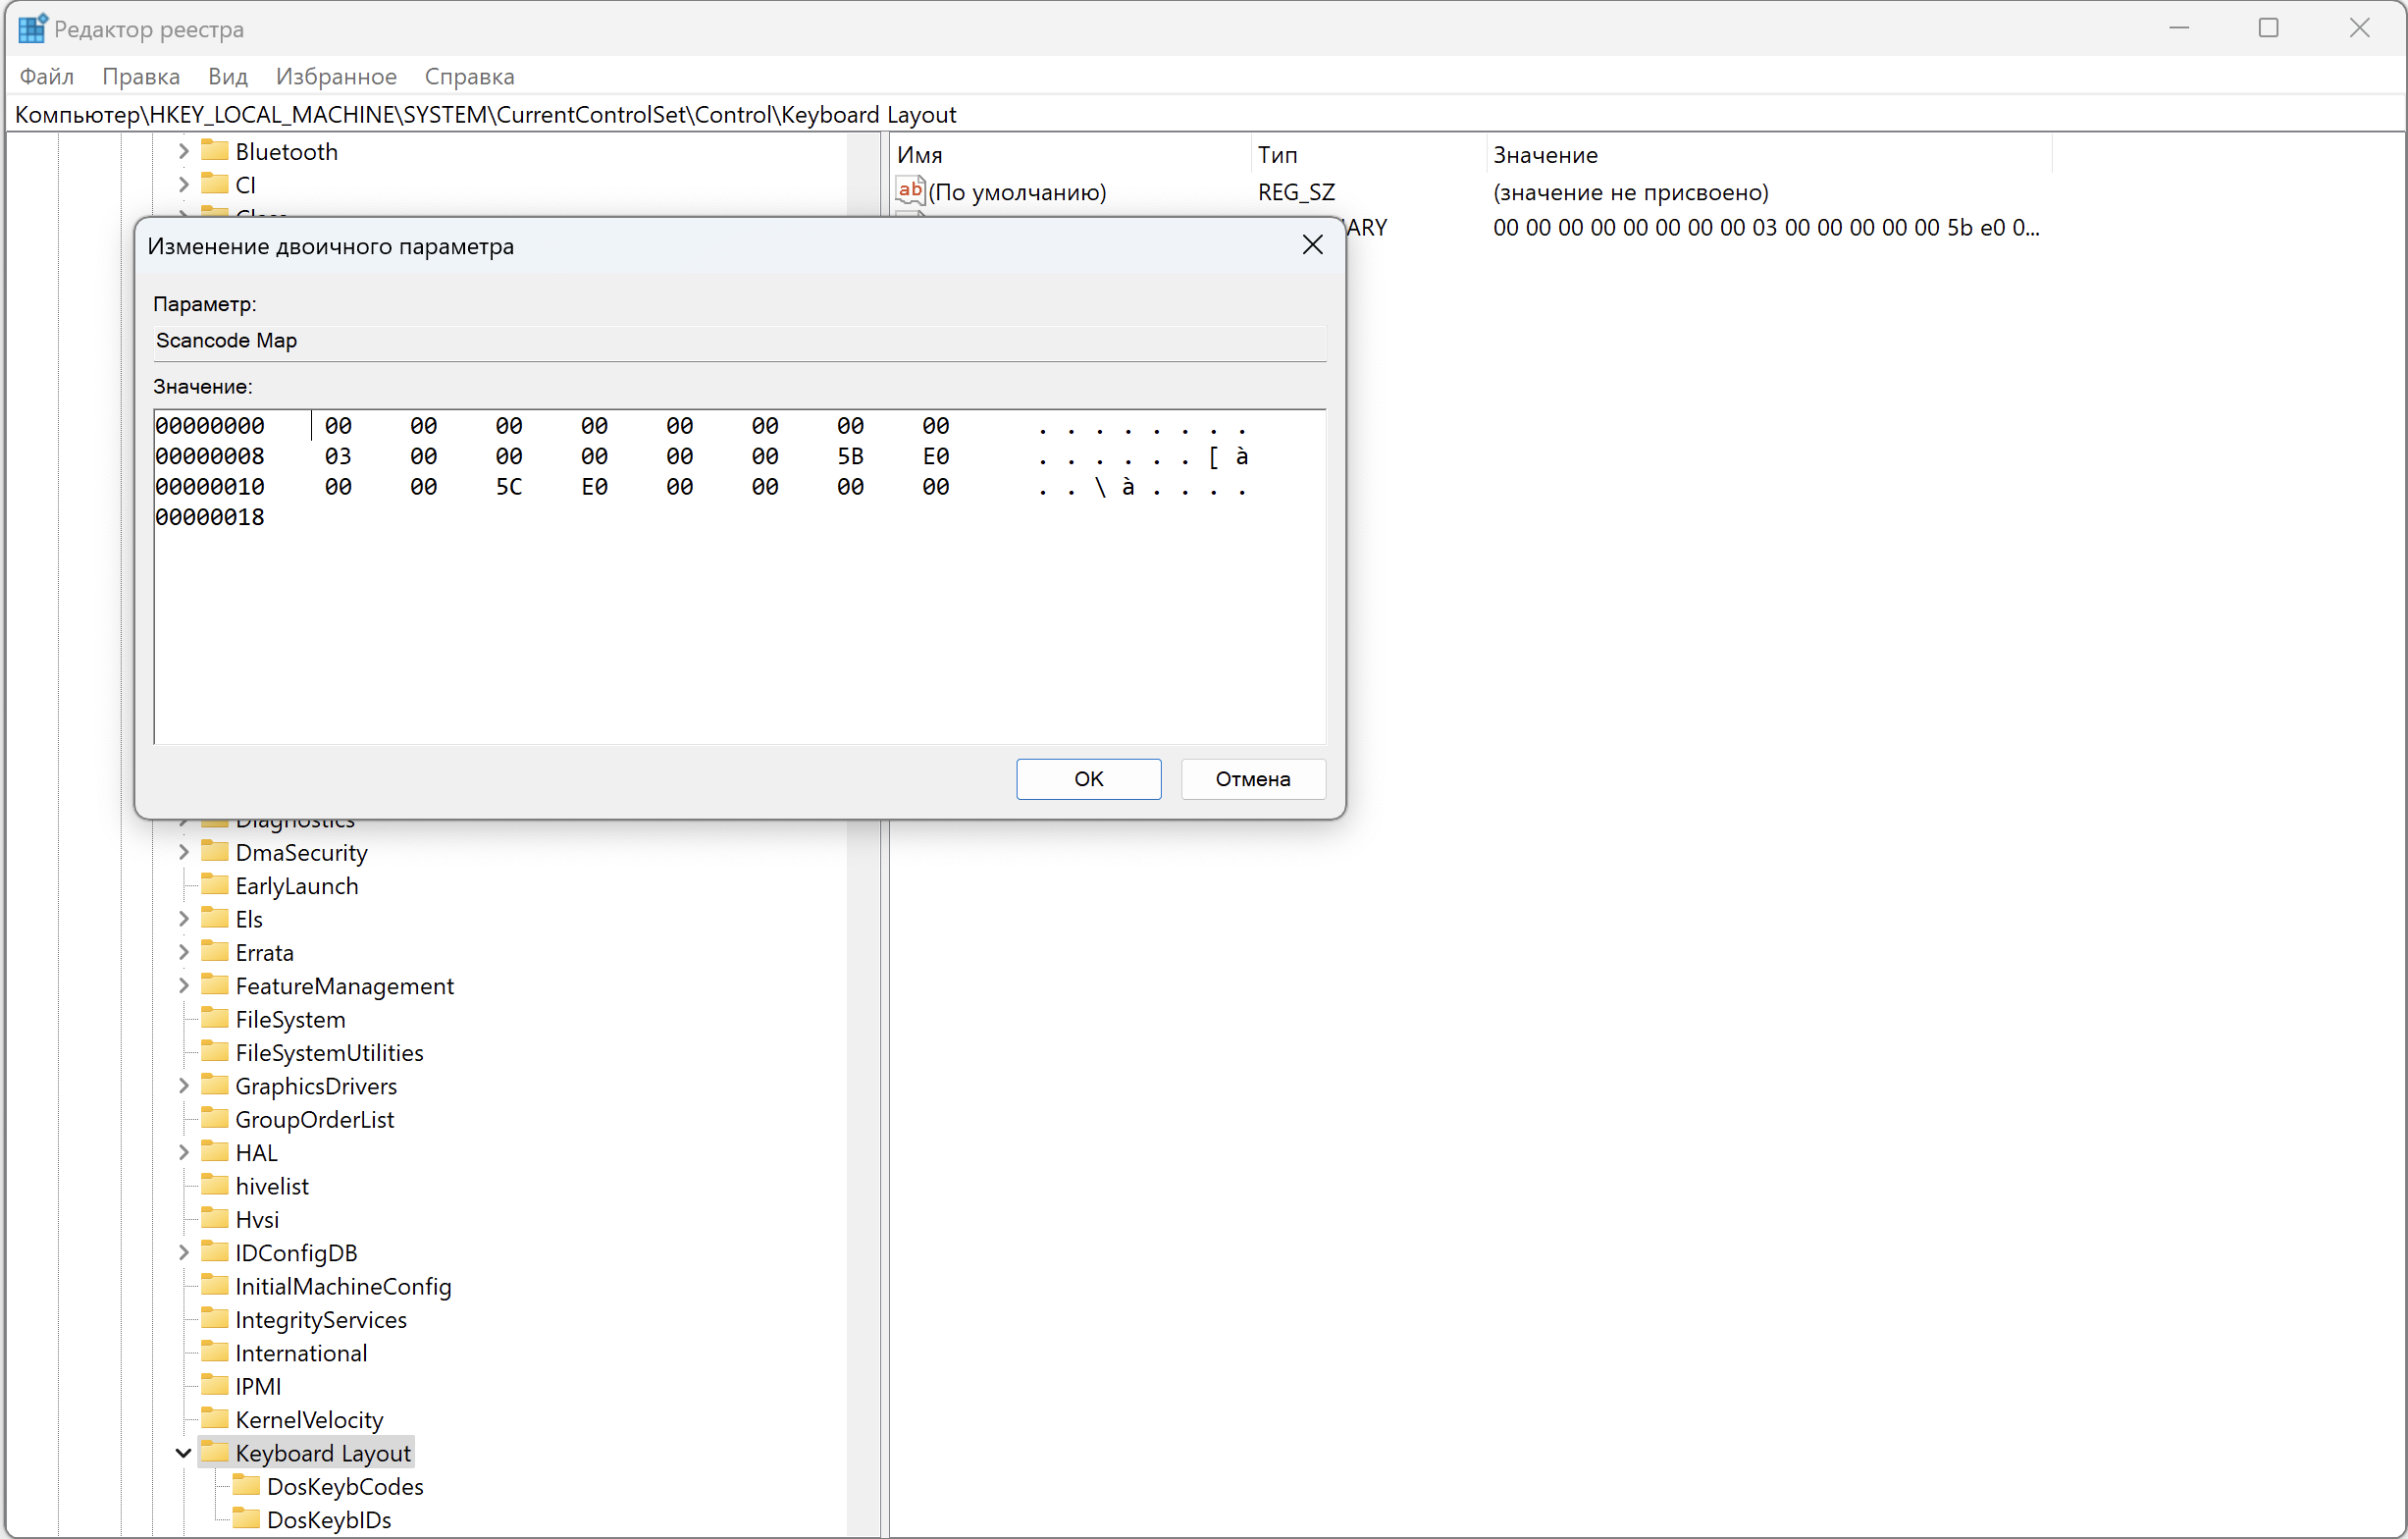
\includegraphics[width=0.8\textwidth]{../images/regedit_scancode_map.png}
                        \caption{Отключение клавиши Win}
                    \end{figure}
          \end{itemize}
          }
    \item {Перезагрузите компьютер:
          \begin{itemize}
              \item После внесения изменений перезагрузите компьютер, чтобы изменения вступили в силу.
          \end{itemize}}
    \item {Чтобы востановить клавишу Win удалите ключ Scancode Map из реестра}
\end{enumerate}
\nchapter{Заключение}
В ходе выполнения лабораторной работы были изучены основные ветви системного реестра Windows, их структура, права доступа и способы управления ими. Были рассмотрены различные методы открытия редактора реестра, а также изучены основные учетные записи и группы, участвующие в управлении доступом к реестру.

Кроме того, были рассмотрены способы восстановления реестра, включая использование резервных копий, утилиты SFC, точек восстановления системы и сброса системы. Эти методы позволяют эффективно восстановить работоспособность системы в случае повреждения реестра.

Также были выполнены практические задания по настройке системы через реестр, такие как включение механизма Prefetcher только для загрузки системы, увеличение скорости выключения компьютера и деактивация клавиши Win. Эти настройки демонстрируют возможности реестра в настройке работы операционной системы Windows.

Таким образом, работа позволила не только изучить структуру реестра, но и приобрести практические навыки по настройке системы с его помощью.
\end{document}
